\documentclass{beamer}
\usepackage{beamerthemesplit} % new 
\usepackage{graphicx}
\usepackage{caption}
%\usepackage{subcaption}
\usepackage{lmodern}
\usepackage{color}
\usetheme{Pittsburgh}
\usepackage{amsmath}
\usecolortheme{dolphin}
\usepackage{marvosym}
% citations
\usepackage[]{natbib}
\usepackage{appendixnumberbeamer}

\usepackage{etoolbox}
\makeatletter
\patchcmd{\beamer@section}
  {\def\insertsectionhead{\hyperlink{Navigation\the\c@page}{#1}}}
  {\protected@edef\insertsectionhead{\noexpand\hyperlink{Navigation\the\c@page}{#1}}}
  {}{}
\patchcmd{\beamer@subsection}
  {\def\insertsubsectionhead{\hyperlink{Navigation\the\c@page}{#1}}}
  {\protected@edef\insertsubsectionhead{\noexpand\hyperlink{Navigation\the\c@page}{#1}}}
  {}{}
\makeatother

\AtBeginSection[]
{
  \begin{frame}<beamer>
    \frametitle{Topics}
    \tableofcontents[currentsection,currentsubsection]
  \end{frame}
}

\AtBeginSubsection[]
{
  \begin{frame}<beamer>
    \frametitle{Topics}
    \tableofcontents[currentsection,currentsubsection]
  \end{frame}
}


\title[Market Design Exp. Finance]{Market Design in Experimental Finance}
\author[L\'opez Vargas]{Kristian L\'opez Vargas\inst{1}}
\institute[UCSC]{\inst{1} Economics Department, University of California, Santa Cruz  }
\useoutertheme{infolines}

\begin{document}

\date{BEEC 2020 - Bogotá} 

\hypertarget{start}{}

\frame{\titlepage} 

\section{Summary}
\frame{\frametitle{One-Slide Summary}
\begin{itemize}
\item \textbf{Introduction}: 
\begin{enumerate}
    \item Basics on Market Design
    \item Three Main Advances
    \item Sniping in non-financial contexts
\end{enumerate}
% \pause

\item \textbf{Market design in Financial Markets}: 
\begin{enumerate}
    \item High Frequency Trading (HFT)
    \item Algorithmic Trading
    \item Consequences of the Market Design
\end{enumerate}
% \pause

\item \textbf{Alternatives for the Standard Financial Market Designs}:

\begin{enumerate}
    \item Speed Bumps
    \item Frequent Batch Auctions
    \item Continuous Scaled Limit Orders
\end{enumerate}

\item \textbf{Conclusions}

\end{itemize}
}

\section{Introduction}
\frame{\frametitle{Basics on Market Design}
\begin{itemize}
    \item By \textbf{market design}, we are talking about the institutions and allocation rules of many economic environments
    \begin{enumerate}
        \item Marketplaces
        \item Auctions
        \item Centralized allocations, etc
    \end{enumerate}
    \item Some examples:
    \begin{itemize}
        \item[-] Auctions for spectrum, electricity, and other commodities
        \item[-] Tradable permit systems for pollution abatement and other environmental regulations
        \item[-] Online reputation and feedback systems
    \end{itemize}
    \item How can we \textbf{research} about them?: Observing the \textbf{performance} of a new market design on simple situations created in the \textbf{lab}
\end{itemize}
}

% \frame{\frametitle{Three Main Advances}
% \begin{itemize}
%     \item \textbf{Theoretical Research}:
%     \begin{enumerate}
%         \item Incorporation of incomplete information
%         \item Nash equilibrium to incomplete information games
%         \item Conceptualization of “type” of player
%         \item Application of game theory for Industrial Organization
%     \end{enumerate}
%     \item \textbf{Behavioral Economics}:
%     \begin{enumerate}
%         \item \textbf{Isolation errors}: Treat risky projects separately rather than together
%         \item \textbf{House money effect}: More risk seeking in the presence of a prior gain
%         \item \textbf{Break-even effect}: With prior losses, outcomes with a chance to break-even are attractive
%     \end{enumerate}
%     \item \textbf{Laboratory Experiments}: Evaluation of different market designs for multiple homogeneous objects across different environments
% \end{itemize}
% }

\frame{\frametitle{Three Main Advances 1}
\textbf{Theoretical Research}:
\begin{itemize}
    \item At the theoretical level, the most important tool for market design is game theory.
    \item Harsanyi (1967, 1968): Incorporation of any incomplete information without loss of generality as the interim stage of some model of asymmetric information
    \item Extension of Nash's concept of an equilibrium point to games of incomplete information
    \item Concept of a “type” that summarizes all of the relevant characteristics of a particular player
    \item The first applied area of economics that embraced game theory was industrial organization (bargaining, contract design, pricing, etc.)
\end{itemize}
}

\frame{\frametitle{Three Main Advances 2}
\textbf{Behavioral Economics}:
\begin{itemize}
    \item Kahneman and Tversky (1979): two central aspects of choice under uncertainty: loss aversion and the probability weighting function
    \item Kahneman and Lovallo (1993): “isolation errors”, whereby people tend to treat risky prospects separately rather than together, as the third component in risky choice
    \item Application in the context of managerial decision-making (e.g., the pervasiveness of small-scale insurance policies and the equity premium puzzle)
    \item Thaler and Johnson (1990):
    \begin{enumerate}
        \item “House money effect”, whereby decision makers become more risk seeking in the presence of a prior gain
        \item “Break-even effects”, whereby, in the presence of prior losses, outcomes which offer a chance to break even are especially attractive
    \end{enumerate}
\end{itemize}
}

\frame{\frametitle{Three Main Advances 3}
\textbf{Laboratory Experiments}:
\begin{itemize}
    \item Katok and Roth (2004) investigate in the laboratory the performance of two “Dutch” auctions for selling multiple homogenous objects:
    \begin{enumerate}
        \item the ascending auctions used in eBay, and
        \item the flower auctions in the Netherlands
    \end{enumerate}
    \item Descending auctions perform well across environments, while the eBay ascending auction better avoids the free-riding problem
    \item Significant implications for market design for procurement and privatization
    \item  Alvin Roth and Lloyd Shapley received the 2012 Nobel Prize in Economics “for the theory of stable allocations and the practice of market design” 
\end{itemize}
}

\frame{\frametitle{Sniping in non-financial contexts 1}
\begin{itemize}
    \item One area of market design research is concerned with the strategic timing of interaction.
    \item In matching markets, Roth and his coauthors develop mechanisms that address problems arising from incentives to act earlier than others.
    \item Competition for people and positions in various job markets led to very early dates of appointment
    \item For example, in some job markets, students were being hired before useful information about their performance was available and before the students themselves could develop informed career preferences.
    \item Timing is also an important aspect of strategic behavior in auction markets. A strategy called \textbf{“sniping”} is prevalent in many auction market environments, hampering the efficiency of trade.
\end{itemize}
}

\frame{\frametitle{Sniping in non-financial contexts 2}
\textbf{Online auctions}:
\begin{itemize}
    \item Online auctions for consumer goods are often run in continuous time.
    \item The simplest rule for ending such auctions is a fixed end time, as employed by eBay.
    \item On eBay, a substantial fraction of bidders tends to submit their bids in the closing seconds of an auction, which is called “sniping”.
    \item Bidding is different on other platforms such as those formerly run by Amazon.
    \item Amazon auctions were automatically extended if necessary past the scheduled end time until 10 minutes passed without a bid.
\end{itemize}
}

\frame{\frametitle{Sniping in non-financial contexts 3}
\begin{figure}
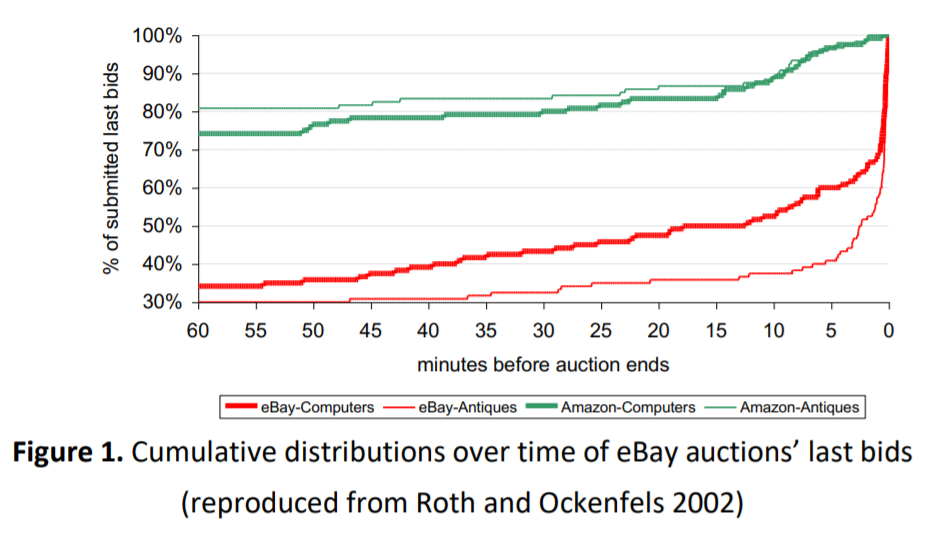
\includegraphics[width=0.9\textwidth]{img/eBay_auctions.PNG}
\end{figure}
}

%%%%%%%%%%%%%%%%%%%%%%%%%%%%%%%%%%%%%

\section{Market Design in Financial Markets}

\frame{\frametitle{Market Design in Financial Markets 1}
\begin{itemize}
    \item \textbf{HFT}: Trading that uses powerful computers to transact a large number of orders within fractions of a second (more than 50\% of traded volume worldwide).
    \item \textbf{Algorithmic Trading}: Decisions are \textbf{encoded} into algorithms which act on their behalf by communicating with the exchange as market conditions change.
\end{itemize}
}

\frame{\frametitle{Market Design in Financial Markets 2} 
Continuous Double Auction (CDA): 
\begin{itemize}
\item Trade can happen at \textbf{any moment} of time. 
\item Strict \textbf{price, time priority}. 
% \item Market makers: post buy/sell limit orders that remain in the book. 
% \item Takers: submit market orders to transact immediately. 
\end{itemize} 
\textbf{Trading strategies: 
}
\begin{itemize}
\item market maker (also sets a spread)
\item sniper 
\end{itemize}
\textbf{Technology strategy:}
\begin{itemize}
\item Traders can subscribe to faster (lower-latency) communication technology at a cost of $c_{speed}$ per second.
\end{itemize}
\centering 
\textbf{There is value to reacting faster to public signal} \\
}


\frame{\frametitle{Market Design in Financial Markets 2} 
\begin{itemize}
\item Continuous limit order book markets violate basic asset pricing principles at high-frequency time horizons.
\item That is, the \textbf{continuous market does not actually "work" in continuous time}.
\item The next figures depict the price paths of the two largest financial instruments that track the S\&P 500 index (tickers SPY and ES) on a trading day in 2011.
\item The two instruments are nearly perfectly correlated over the course of the trading day, as we would expect given the near-arbitrage relationship between them.
\item Even nearly perfectly correlated over the course of an hour or a minute
\item When we zoom in to high-frequency time scales, we see
that the \textbf{correlation breaks down}; this leads to \textbf{arbitrage opportunities}.
\end{itemize}
}

\frame{
\begin{figure}
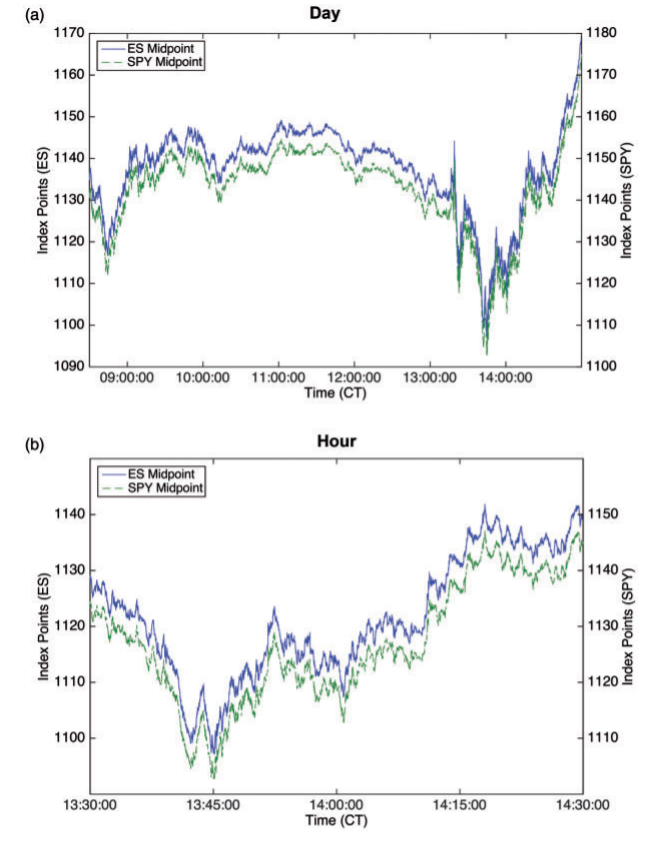
\includegraphics[width=0.45\textwidth]{img/corr_dayhour.PNG}
\caption{ES and SPY Time Series at Human-Scale and High-Frequency Time Horizons (extracted from Budish et al. (2015)).}
\end{figure}
}

\frame{
\begin{figure}
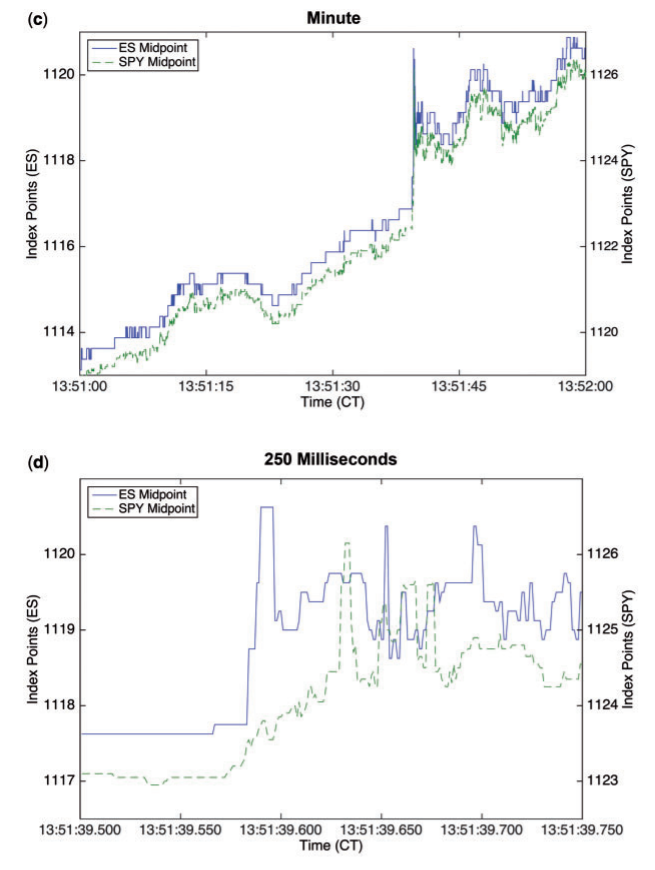
\includegraphics[width=0.45\textwidth]{img/corr_minutesms.PNG}
\caption{ES and SPY Time Series at Human-Scale and High-Frequency Time Horizons (extracted from Budish et al. (2015)).}
\end{figure}
}

\frame{\frametitle{Market Design in Financial Markets 4} 

\begin{enumerate}
    \item Investor arrivals, value jumps in the CDA, sniping, profits.
    \item Equilibrium: N-1 snipers; 1 maker with $S>0$; all fast. \hyperlink{CDA_Equil}{\beamergotobutton{Detail}}
\end{enumerate}

\begin{figure}
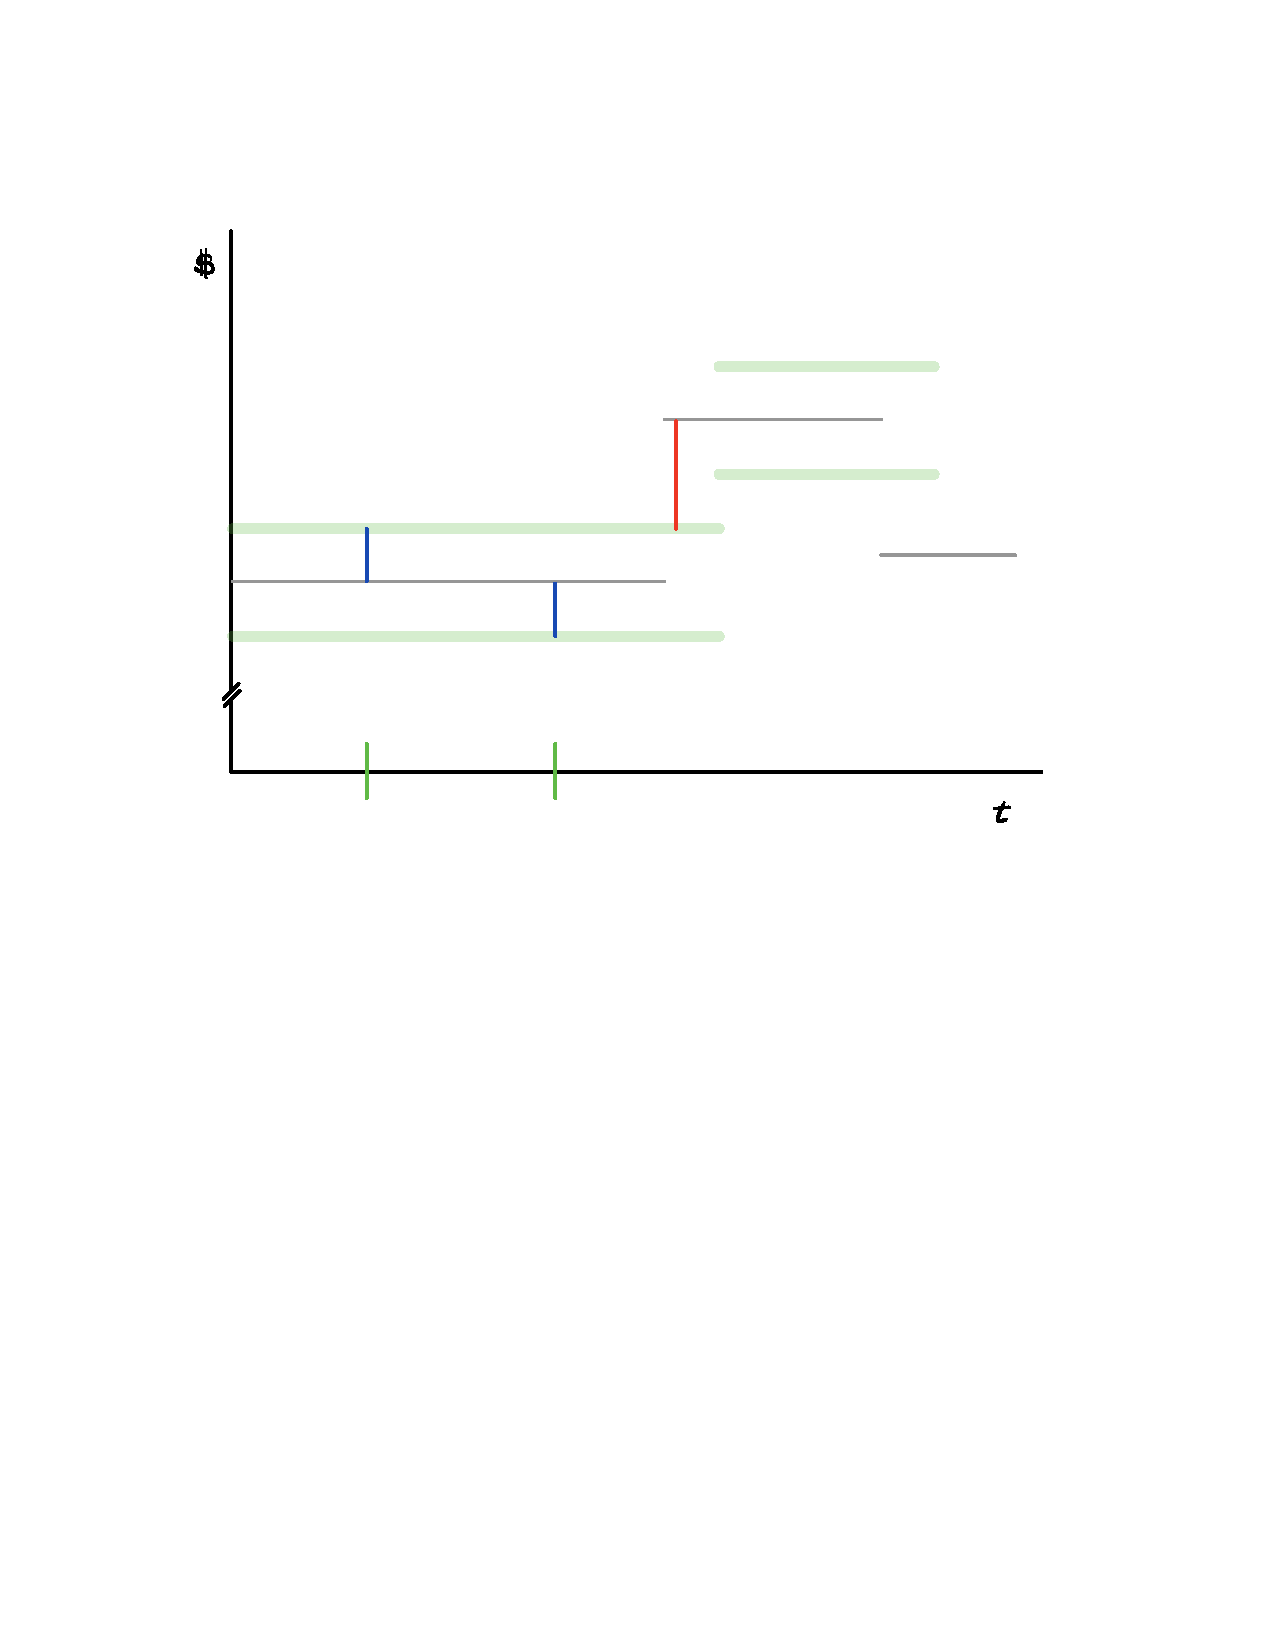
\includegraphics[width=0.6\textwidth]{img/CDA_diagram_events.pdf}
\end{figure}
}

\frame{\frametitle{Market Design in Financial Markets 5}
\begin{itemize}
    \item Their market design have a profound impact on a very specific strategy that hampers the efficiency of trade: \textbf{sniping}
    \item \textbf{Sniping}: Bidding as early or as late as possible to gain an advantage
    \item There is a \textbf{never-ending arms race} for \textbf{faster trading}, which happens because of two market failures in the design:
    \begin{enumerate}
        \item \textbf{Trading in Continuous time}: Causes divergence at high frequencies, which creates \textbf{arbitrage} opportunities
        \item \textbf{Equally attractive orders processed by arrival time}: Incentives for whomever snaps those opportunities faster
    \end{enumerate}
    \item The outcome: a \textbf{massive prisoner's dilemma}
    \item As a consequence, \textbf{alternative} designs have been proposed to \textbf{solve} the issues the \textbf{standard} model causes
\end{itemize}
}

%%%%%%%%%%%

\section{Alternatives for the Standard Financial Market Design}

\begin{frame}{Market Alternative 1: Speed bumps}

\begin{itemize}
    \item \textbf{Speed bumps}: intentional delays between the receipt and execution of (a subset of) trading orders submitted to the exchange.
    \item Easy way to implement change to market design, contrary to proposals like BCS or Kyle-Lee
    \item Menkveld and Zoican (2017) propose a model to analyze the impact of exchange latency on liquidity in the presence of market makers and short-term speculators.
    \item They consider two opposite effects:
    \begin{enumerate}
        \item (+) a faster market allows high-frequency market makers to update their price quotes faster on new information, but
        \item (-) it enables high-frequency speculators to act faster on this new information and profit by sniping potentially stale quotes.
    \end{enumerate}
    \item The model's net effect depends on the ratio of news intensity (+) and liquidity trade intensity (-).
\end{itemize}

\end{frame}

\begin{frame}{Market Alternative 1: Speed bumps}

\begin{itemize}
    \item The \textbf{Investor's Exchange (IEX)} market format is a continuous double auction that implemented, in 2016, a constant 350 microseconds delay on all orders.
    \item This delay is long enough to allow the system a fresh view of the new best bids and offers and to reprice "pegged" orders ahead of snipers.
    \item \textbf{"Pegged" orders}: Previously submitted hidden liquidity-providing orders
    \item As a result, pegged orders are protected from fast traders who would profit from transacting at stale prices when the new best bids and offers changes.
\end{itemize}

\end{frame}

\begin{frame}{Market Alternative 1: Speed bumps}

\begin{itemize}
    \item Aldrich and Friedman (2019) develop a model that captures the essential elements of HFT-inspired reforms at \textbf{IEX}.
    \item That is, they develop an equilibrium model that spotlights the consequences of imposing a uniform delay on new orders while “pegged” orders are automatically repriced without delay.
    % \item In equilibrium, a messaging delay that protects pegged orders will, under a wide range of exogenous parameter values, result in
    % \begin{itemize}
    %     \item a substantially higher proportion of pegged orders,
    %     \item a lower sniper/maker ratio,
    %     \item transactions prices that deviate less from fundamental value
    %     \item lower transactions costs, but
    %     \item higher queuing cost
    % \end{itemize}
    \item Using data provided by IEX during December 2016, they validate and calibrate their model.
    \item By simulating the impact of order protection, they find that order protection
    \begin{itemize}
        \item substantially increases equilibrium pegged orders,
        \item substantially reduces transaction costs, however
        \item queuing costs increase.
    \end{itemize}
    \item Opportunities to profit from dynamic choice of pegged vs market orders are small and fleeting.
\end{itemize}

\end{frame}

\begin{frame}{Market Alternative 1: Speed bumps}

\begin{itemize}
    \item According to Khapko and Zoican (2019), there are \textbf{different designs of speed bumps}, which yield different equilibrium predictions.
    \begin{itemize}
        \item[-] A \textit{deterministic and symmetric} speed bump (IEX) shifts market activity uniformly in the future.
        \item[-] A \textit{deterministic but asymmetric} speed bump, where market makers can cancel orders without delay, leads to lower investments in trading speed.
        \item[-] An \textit{asymmetric and random} speed bump has the potential to stimulate investment in low-latency technology and amplify the arms’ race.
    \end{itemize}
    \item The authors design a laboratory experiment and find that the design of the speed bump is crucial: asymmetric ones reduce low-latency investment by 20\%, whereas symmetric ones have little impact.
    \item The size of speed bump also matters: increasing the speed bump magnitude by one standard deviation (for an asymmetric, deterministic delay) reduces investment by a further 8.33\%.
\end{itemize}

\end{frame}


%%%
\frame[label={FBA}]{\frametitle{Market Alternative 2: The FBA} 
Frequent Batch Auctions (FBA) (Budish et al., 2015)
\begin{itemize}
\item Trading day is divided in \textbf{many uniform price double auctions}
\item Trade does NOT happen at any moment of time, but \textbf{periodically} (say, each tenth of a second), with a batching period for each auction.
\item All trade requests received during the same interval are treated as having arrived at the same (discrete) time.
\item At the end of the batching period, supply and demand cross and \textbf{market clears}. 
 \item Strategy space is the same as in the CDA. 
\end{itemize}
}

\frame[label={FBA}]{\frametitle{Market Alternative 2: The FBA}
\begin{itemize}
\item Discrete time substantially reduces the value of a tiny speed advantage, which eliminates the arms race.
\item In the frequent batch auction market, if multiple traders observe the same information at the same time, they are forced to compete on price instead of speed.
\item BCS supporters claim that this solution attacks the root market design flaw, and not only its symptoms.
\end{itemize}

\begin{figure}
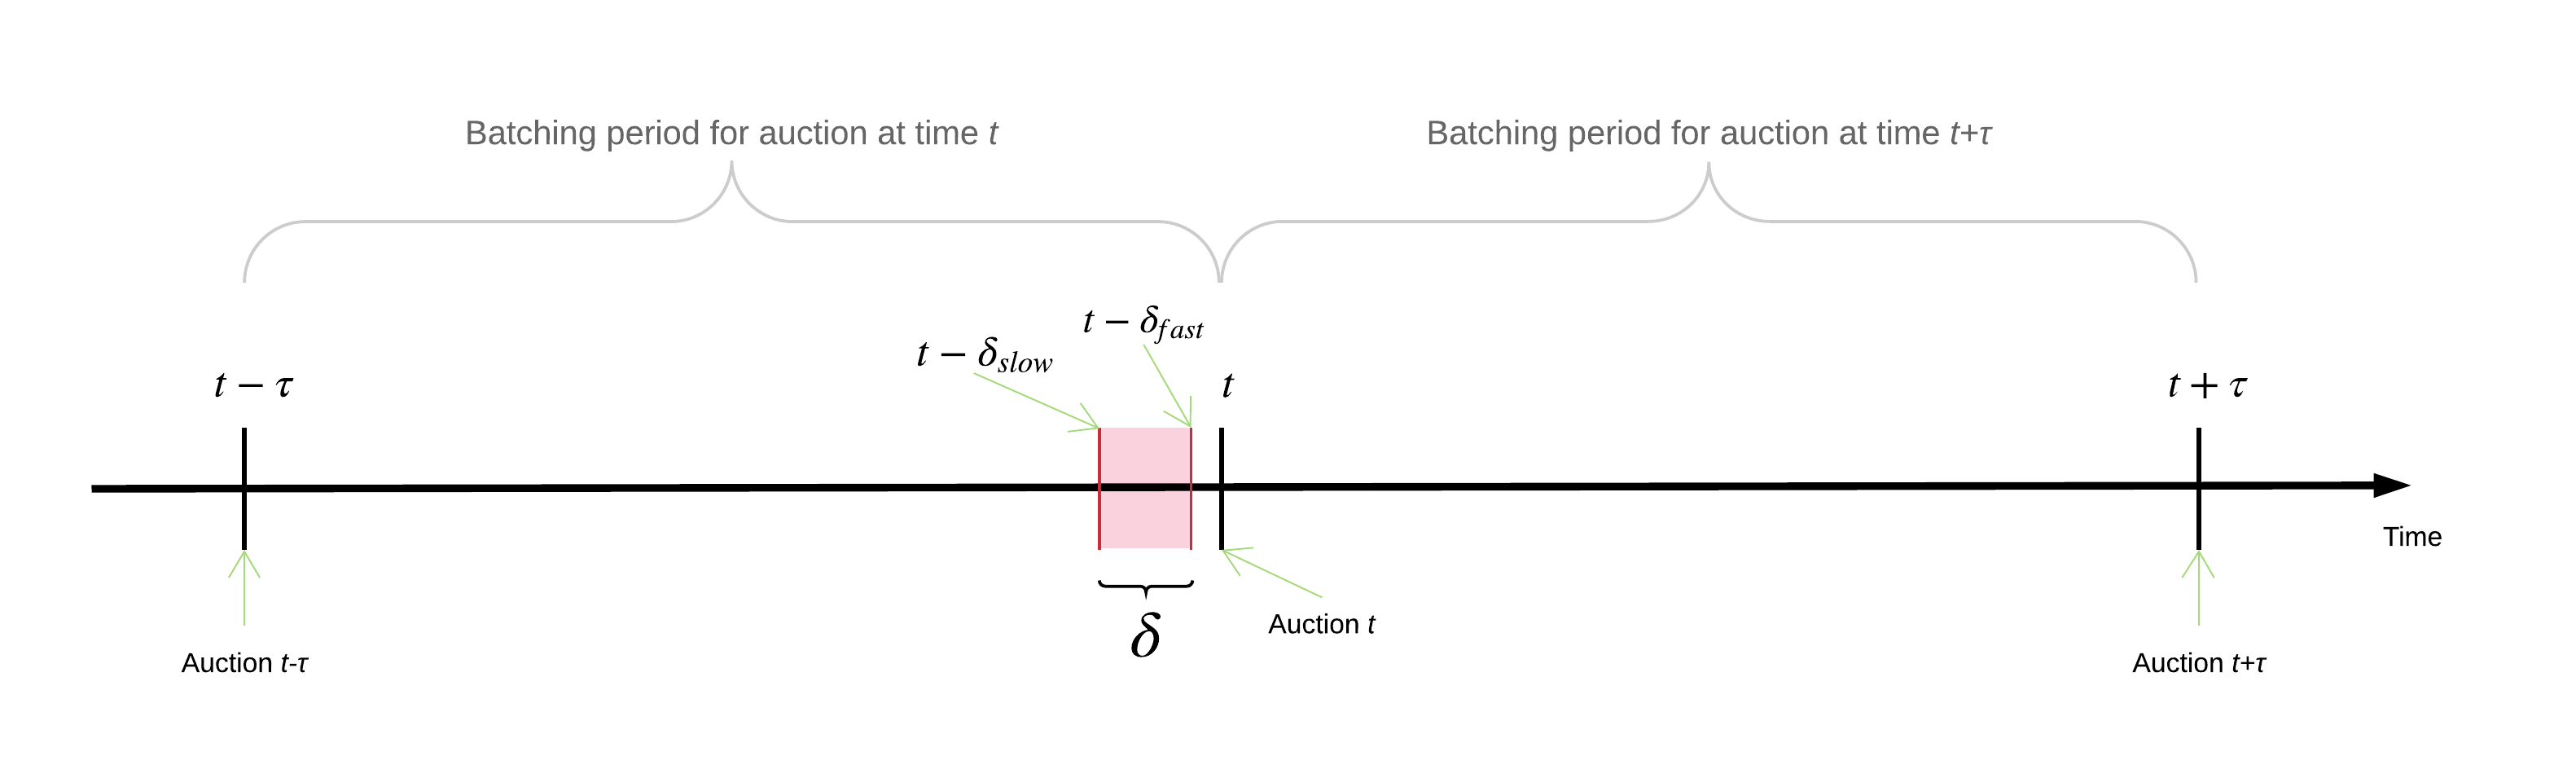
\includegraphics[width=0.8\textwidth]{img/timing_FBA.png}
\caption{\label{fig:FBAtiming}Timing in the FBA format (adapted from Budish et al. (2015)).}
\label{fig:fbaDiagram}
\end{figure}
}

\frame{\frametitle{Market Alternative 2: The FBA} 
Equilibrium: No snipers, everyone is \textit{maker} with $S=0$; all slow.
\hyperlink{FBA_Equil}{\beamergotobutton{}}
\begin{figure}
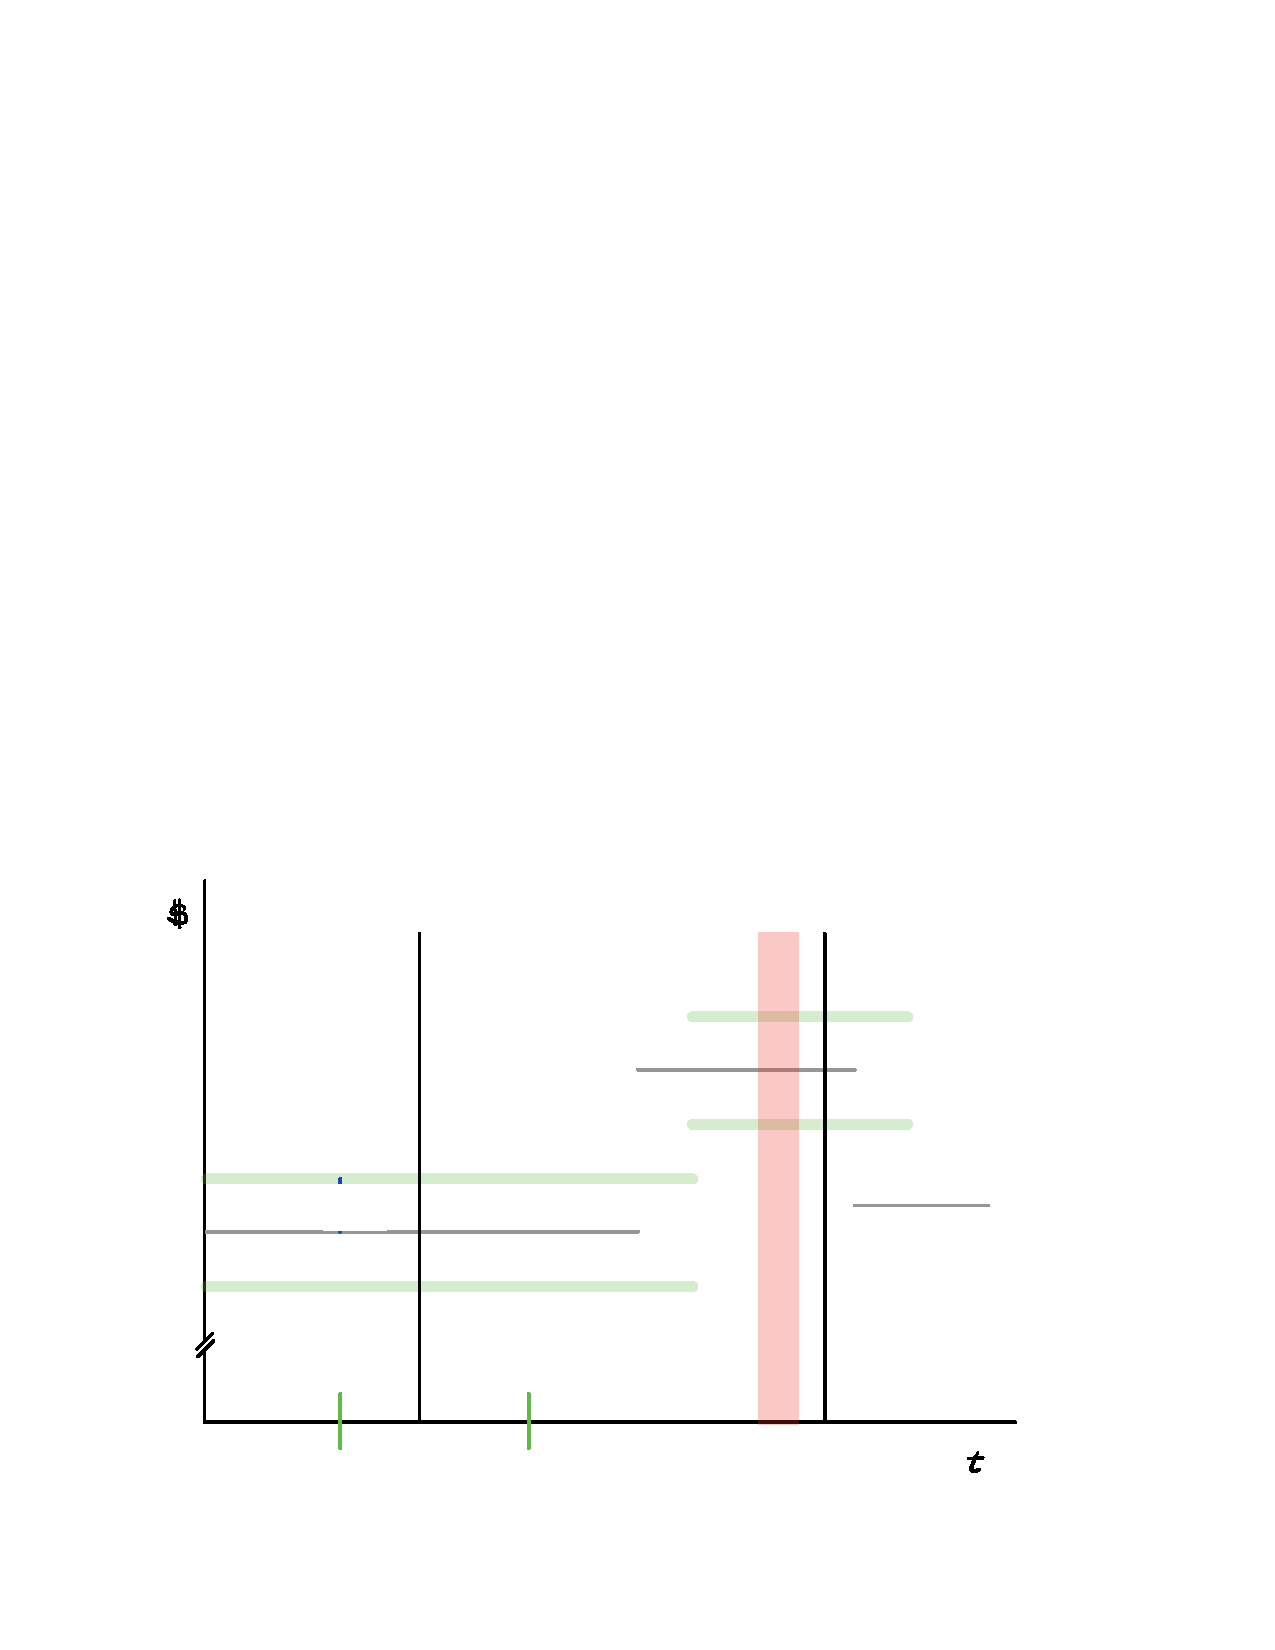
\includegraphics[width=0.7\textwidth]{img/FBA_diagram_events.pdf}
\end{figure}
}

\frame{\frametitle{Experimental Comparisons: Aldricht, Lopez-Vargas (2019)}
\begin{itemize}
\item \textbf{Broad Motivation:} What is a good design for financial markets in the presence of HFT? 
% Does the CDA/CLOB exhibit important flaws? What are the alternative market formats? 
%\hyperlink{motivationDetail}{\beamerbutton{\Coffeecup}}

% \pause
\item \textbf{This paper:} A laboratory study that compares the CDA against the (newly) proposed Frequent Batch Auction (FBA). 

% \pause
\item \textbf{Results:} The FBA outperforms the CDA.

\begin{enumerate}
\item less \textbf{predatory} trading behavior.
\item less \textbf{wasteful investments} in technology.
\item lower \textbf{transacting costs} (market spread)
\item lower \textbf{volatility}, 
\item higher market \textbf{stability}
\end{enumerate}

\end{itemize}
}

%3.1 Subject choices
\frame{ 
\begin{figure}
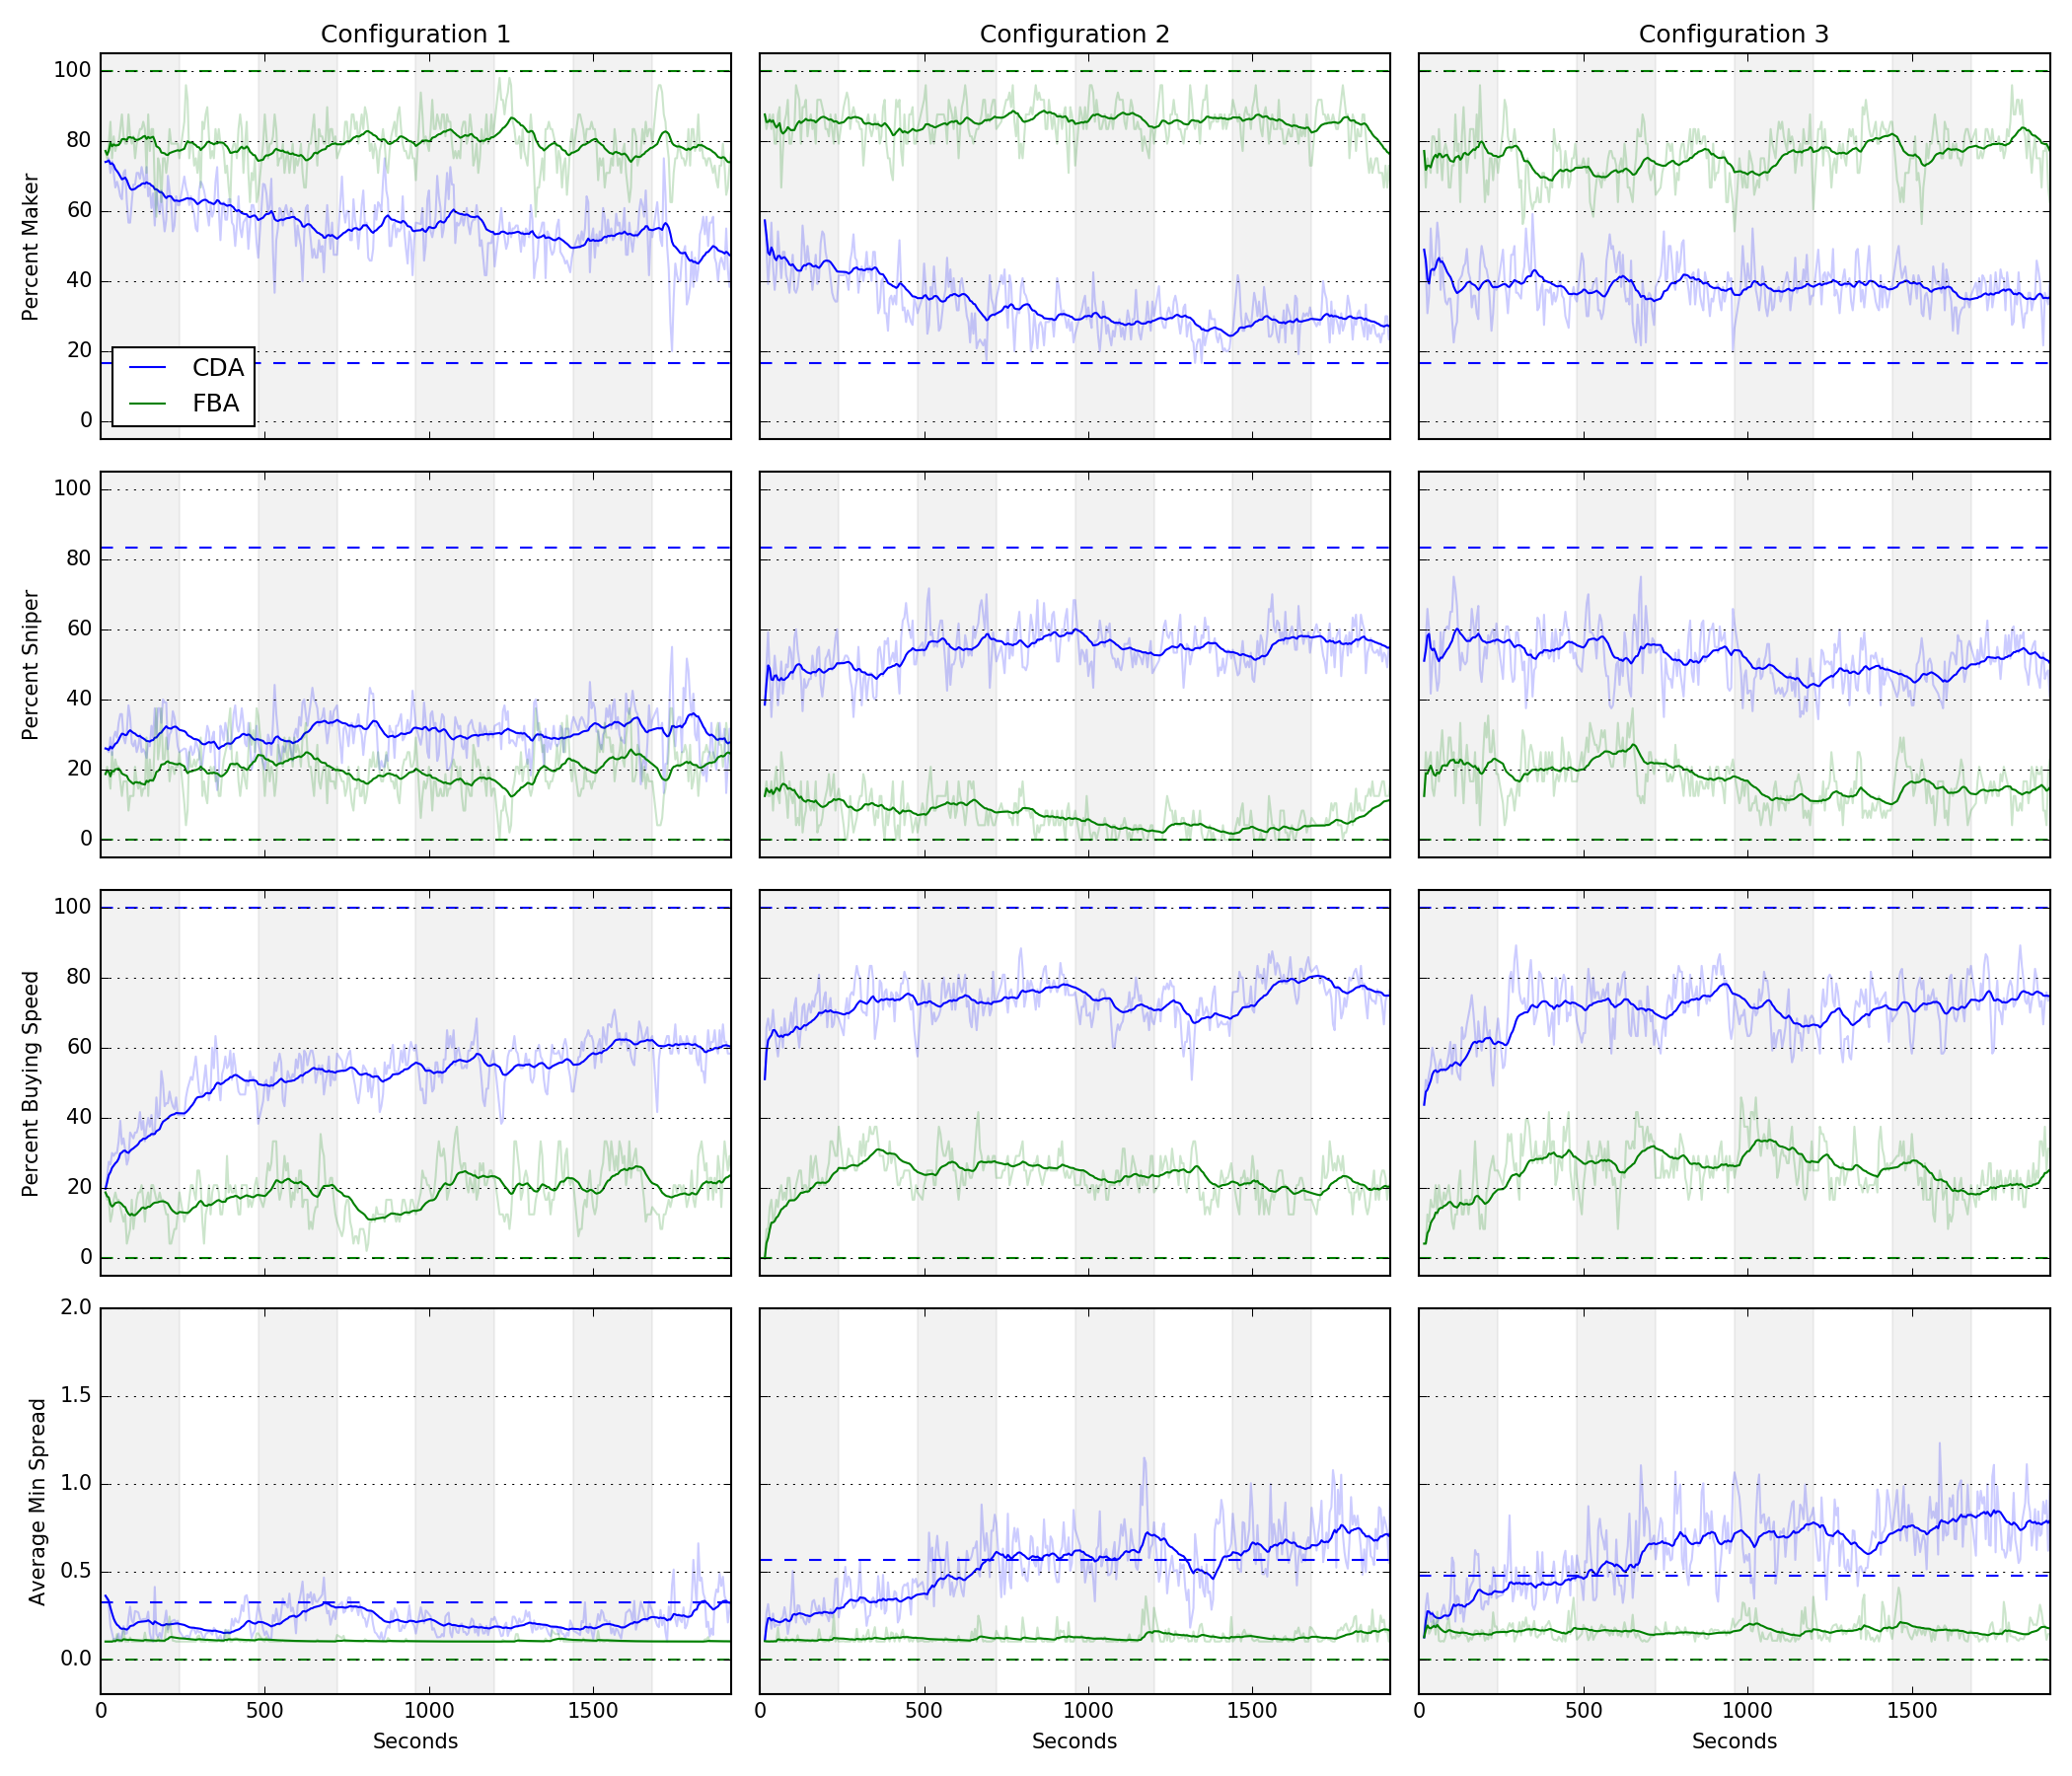
\includegraphics[width=0.70\textwidth]{img/allPlots.png}
\end{figure} 
Rows: \% Maker, \% Sniper, \% Speed, Spread \\
Cols: Market Configs 1, 2, 3.
}

%%%
\frame{\frametitle{Market Alternative 3: CSLO}
Continuous Scaled Limit Orders (Kyle and Lee, 2017)
\begin{itemize}
    \item The \textbf{continuous scaled limit orders} make trading continuous in price, quantity and time
    \item A continuous scaled limit order have two additional parameters that standard limit orders do not have:
    \begin{enumerate}
        \item two price levels $P_L$ and $P_H$ (with $P_L<P_H$), and
        \item a maximum trading speed $U_{max}$.
    \end{enumerate}
    \item Message: ``Buy up to a cumulative total of $Q_{max}$ (shares) at maximum rate $U_{max}$ (shares per hour) at prices between $P_L$ and $P_H$ (dollars per share).''
    \item A trader could mimic a continuous scaled limit order by sending a sequence of very small standard limit orders one at a time, with a new small order sent to replace the previous order after it is executed.
\end{itemize}
}

\frame{
\begin{figure}
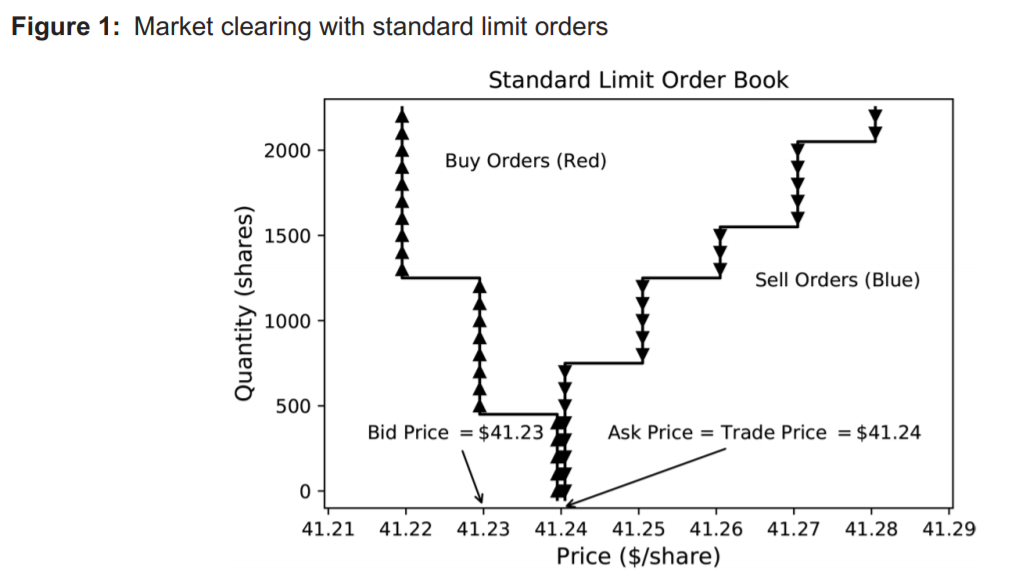
\includegraphics[width=0.9\textwidth]{img/SLO.PNG}
\end{figure}
}

\frame{
\begin{figure}
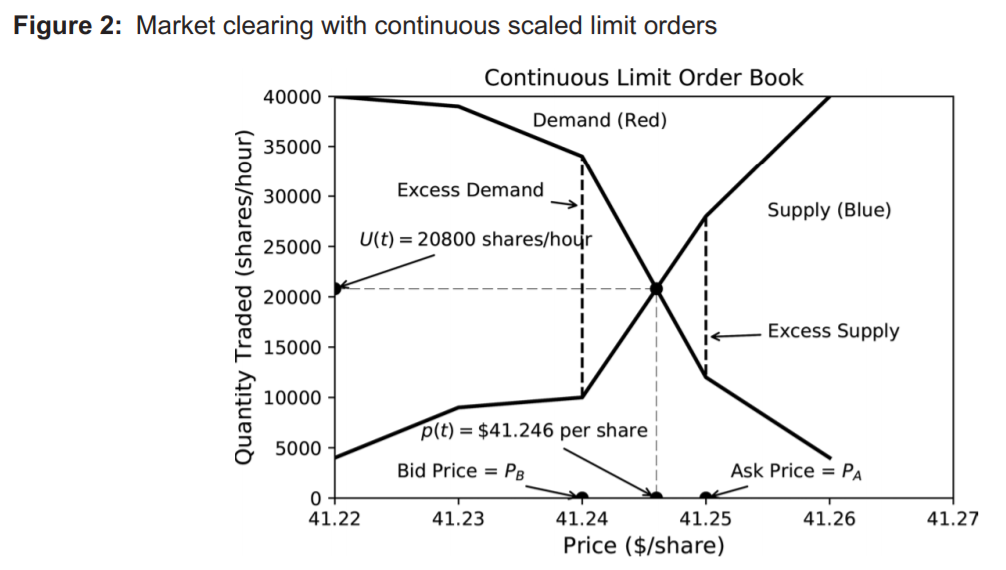
\includegraphics[width=0.9\textwidth]{img/CSLO.PNG}
\end{figure}
} 

\frame{\frametitle{Market Alternative 3: CSLO}
\begin{itemize}
    \item In sum, CSLOs have two special characteristics that differentiate it from the standard model:
    \begin{enumerate}
        \item \textbf{Maximum rate} at which \textbf{orders} are \textbf{executed} over time
        %: As a consequence, supply and demand become flows over time
        \item The \textbf{actual} execution \textbf{rate} can vary \textbf{continuously} between 0 and the maximum rate
        %: This happens as the price varies between upper and lower prices chosen by the trader and allows the existence of a uniquely market clearing price
    \end{enumerate}
    \item Supply and demand become \textbf{flows} over time
    \item Price varies between upper and lower prices chosen by the trader
    \item \textbf{Rents} earned by \textbf{HFT lower} dramatically, because traders with inferior technology can spread their orders easily over time
    \item Orders make flow demand schedules piecewise linear functions of the price, so there is a unique market clearing price with \textbf{no excess supply or demand} and making unnecessary any allocation rule like time priority.
\end{itemize}
}

\section{Conclusions}

\frame{\frametitle{Conclusions}
\begin{itemize}
    \item Today, economists, computer scientists, managers and others are increasingly asked to design mechanisms for markets and organizations.
    \item Many of the applications are motivated by failures of incentives in markets and organizations.
    \item Even small changes in the rules can have a dramatic impact on the effectiveness and efficiency of a market.
    \item Market design may require decisions that are beyond current knowledge, so it is often fruitfully complemented by \textbf{lab and field experiments}.
    \item New challenges:  computer and communication technology
    \begin{itemize}
        \item[-] Smart markets: dating, kidney exchanges, ad auctions, etc.
    \end{itemize}
\end{itemize}
}

\frame{\frametitle{Main references}
\footnotesize
\begin{itemize}
    \item Aldrich, E., and Friedman, D. (2019). "Order Protection through Delayed Messaging," Available at SSRN: https://ssrn.com/abstract=2999059
    \item Aldrich, E., and López Vargas, K. (2019). "Experiments in high-frequency trading: comparing two market institutions," Experimental Economics, 1-31.
    \item Budish, E., Cramton, P., and Shim, J. (2015), “The High-Frequency Trading Arms Race: Frequent Batch Auctions as a Market Design Response,” The Quarterly Journal of Economics, 130, 1547–1621.
    \item Chen, Y, Cramton, P., List, J., and Ockenfels, A. (2019). "Market Design, Human Behavior and Management," Working Paper, University of Cologne
    \item Khapko, M., and Zoican, M. (2019). "Do speed bumps curb low-latency trading? Evidence from a laboratory market," Available at SSRN: https://ssrn.com/abstract=3351269
    \item Kyle, A., and Lee J. (2017). "Toward a fully continuous exchange," Oxford Review of Economic Policy, 33, 650–675.
    \item Menkveld, A. J. and Zoican, M. A. (2017), “Need for speed? Exchange latency and liquidity,” Review of Financial Studies, 30, 1188–1228.
\end{itemize}
}


%%%%%%%%%%%%%%%%%%%%%%%%%%%%%%%%%%%%%%%%%%%%%%%%
\appendix

\begin{frame}{Appendix}

\end{frame}

\frame{\frametitle{One-Slide Summary}
\begin{itemize}
\item \textbf{HFT}: trading that uses powerful computers to transact a large number of orders within fractions of a second (more than 50\% of traded volume worldwide).
% \pause

\item \textbf{Broad Motivation:} What is a good design for financial markets in the presence of HFT? 
% Does the CDA/CLOB exhibit important flaws? What are the alternative market formats? 
\hyperlink{motivationDetail}{\beamerbutton{\Coffeecup}}

% \pause
\item \textbf{This paper:} A laboratory study that compares the CDA against the (newly) proposed Frequent Batch Auction (FBA). 

% \pause
\item \textbf{Results:} The FBA outperforms the CDA.

\begin{enumerate}
\item less \textbf{predatory} trading behavior.
\item less \textbf{wasteful investments} in technology.
\item lower \textbf{transacting costs} (market spread)
\item lower \textbf{volatility}, 
\item higher market \textbf{stability}
\end{enumerate}

\end{itemize}
}


% \frame{\frametitle{The HFT Debate} 
% \begin{itemize}
% \item Exchanges (NYSE et al.) automated order execution about 20 years ago, substantially reducing spreads and latencies. 
% \item Today, most trades involve low latency, automated traders: the HFT industry.
% \item HFT firms provide liquidity, although not cheaply, and this liquidity may be illusory. Overall, actual transactions costs are not necessarily lowest under the current market design and with HFTs.
% \item HFT firms \textit{might} be destabilizing the markets (as in the 2010 ``flash crash'').
% \item Regulators seem to take these fears seriously, and are considering heavy handed ``fixes''.
% \end{itemize}
% }


% \frame{\frametitle{Environment: Basics} 
% Orders:
% \begin{enumerate}
% \item limit order: example: "BUY, up to \$101, 20 Units, GTC"
% \item market order: example: "BUY, up to $\infty$, 30 Units, IOC"
% \end{enumerate}
% \vspace{5mm}
% Latencies: \\
% Time elapsed between sending and receiving the order, and between receipt and processing.
% }


\frame{\frametitle{BCS Environment: Exogenous Processes} 

\begin{itemize}
    \item Budish, Cramton and Shim (QJE, 2015, hereafter BCS) 
    \item There is one \textbf{single asset}, trades in a single exchange. 
    \pause
    \vspace{.3cm}
    \item Two exogenous processes generate \textbf{incentives to trade}:
\begin{enumerate}

\item the fundamental value of the asset, $V(t)$ 
\begin{itemize}
\item publicly \textbf{observed}
\item follows a \textbf{compound Poisson} jump process
\item arrival rate of $\lambda_V$ per second and jump distribution $F_{V}$
\end{itemize} 


\item a population of investors (noise traders) that
\begin{itemize}
\item arrive at random times with \textbf{Poisson rate} of $\lambda_{I}$ per second, 
\item each places a \textbf{unit market order} to buy or sell with equal probability.
\end{itemize} 

\end{enumerate}
    \item \textbf{Profits} from reversing positions with respect to $V(t)$.
    
% Human participants play the role of trading firms and, at any instant, can choose whether
% \begin{itemize}
% \item to exit the market (out)
% \item to participate as a market maker
% \item or as a sniper
% \end{itemize}

\end{itemize}

}


\frame{\frametitle{BCS Environment: Exogenous Processes} 
\begin{enumerate}
\item Fundamental value V(t) (jump rate $\lambda_V$, $\Delta V$ distributed as $ N(0,\sigma^2)$)
\item Investor arrivals with unit market orders (arrival rate $\lambda_I$, Buy or Sell)
\end{enumerate}

\begin{figure}
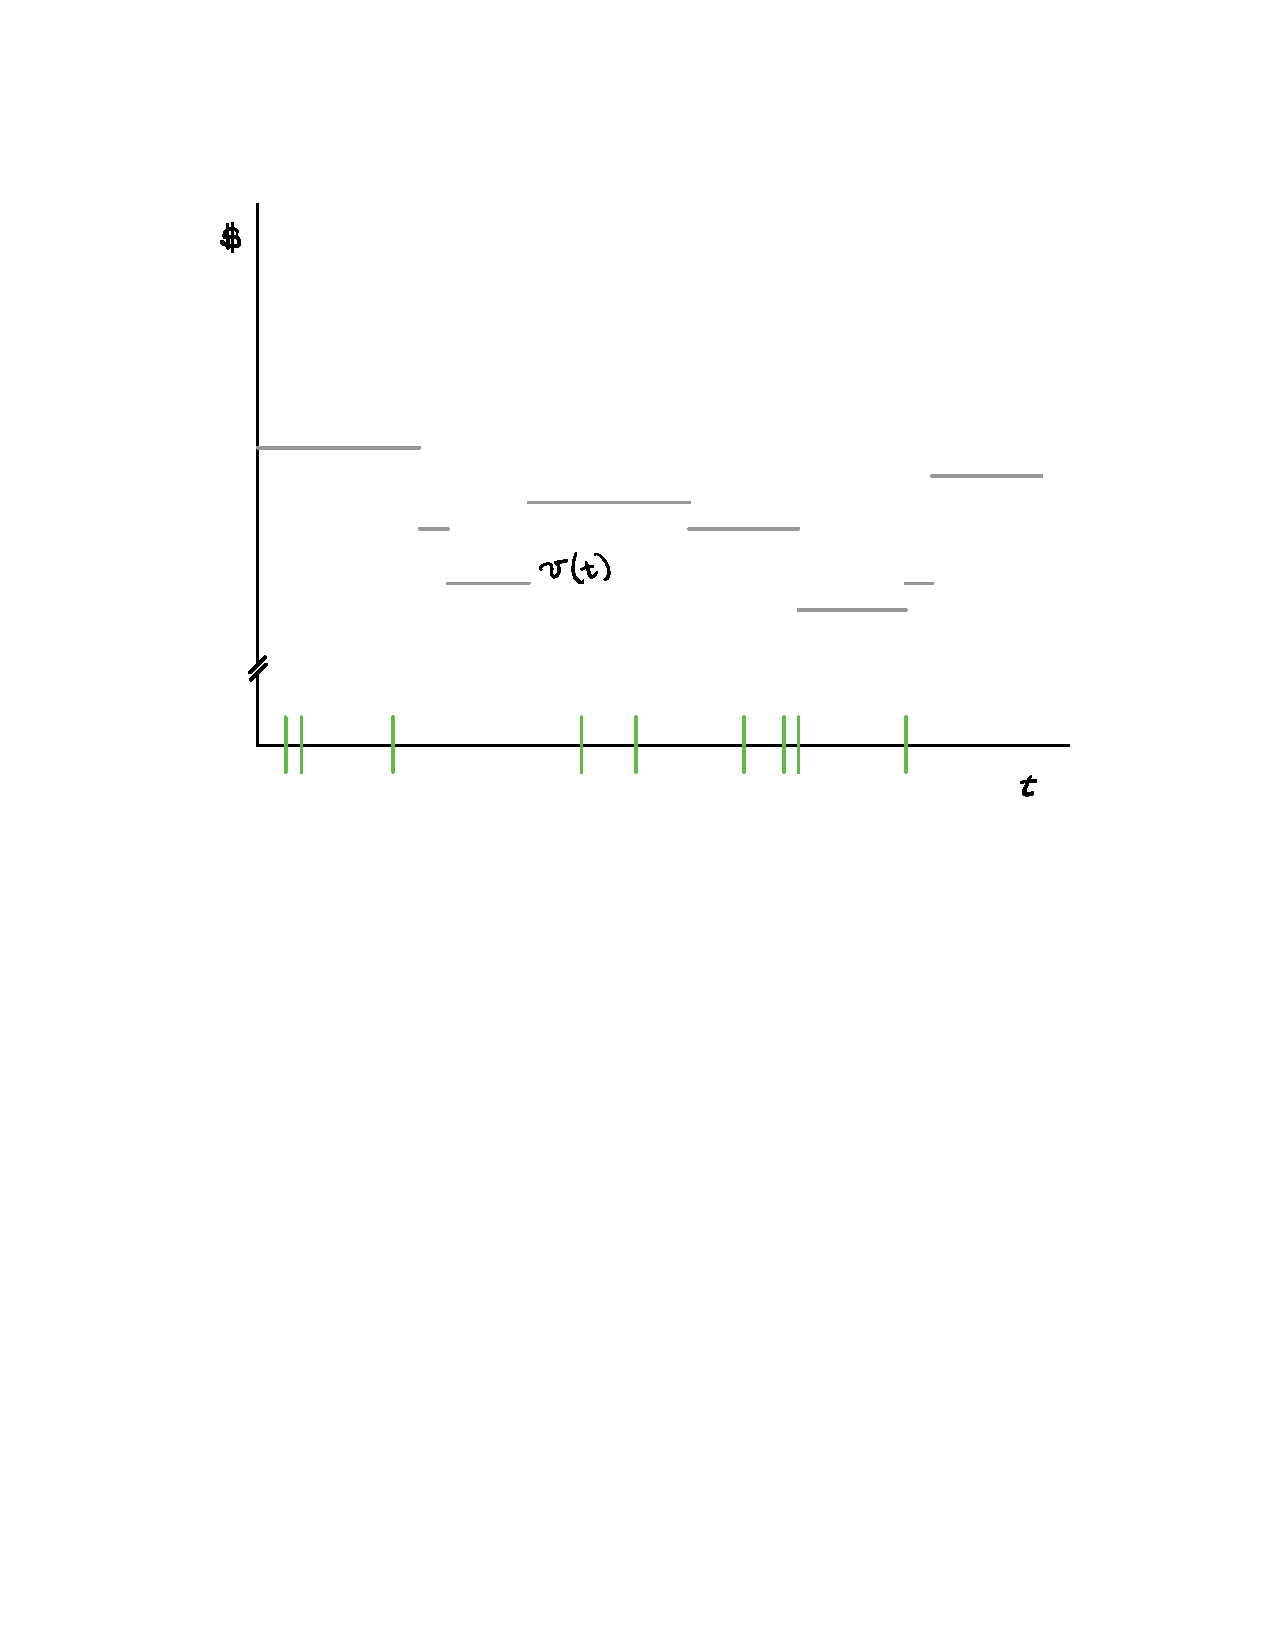
\includegraphics[width=0.7\textwidth]{img/two_processes.pdf}
\end{figure}
} 


\frame{\frametitle{BCS Environment: Orders, Latencies}
\begin{enumerate}
    \item Limit orders, market orders 
    \item Profits against V(t).
    \item There exist latencies: it takes time to send orders (slow / fast).
\end{enumerate}
\begin{figure}
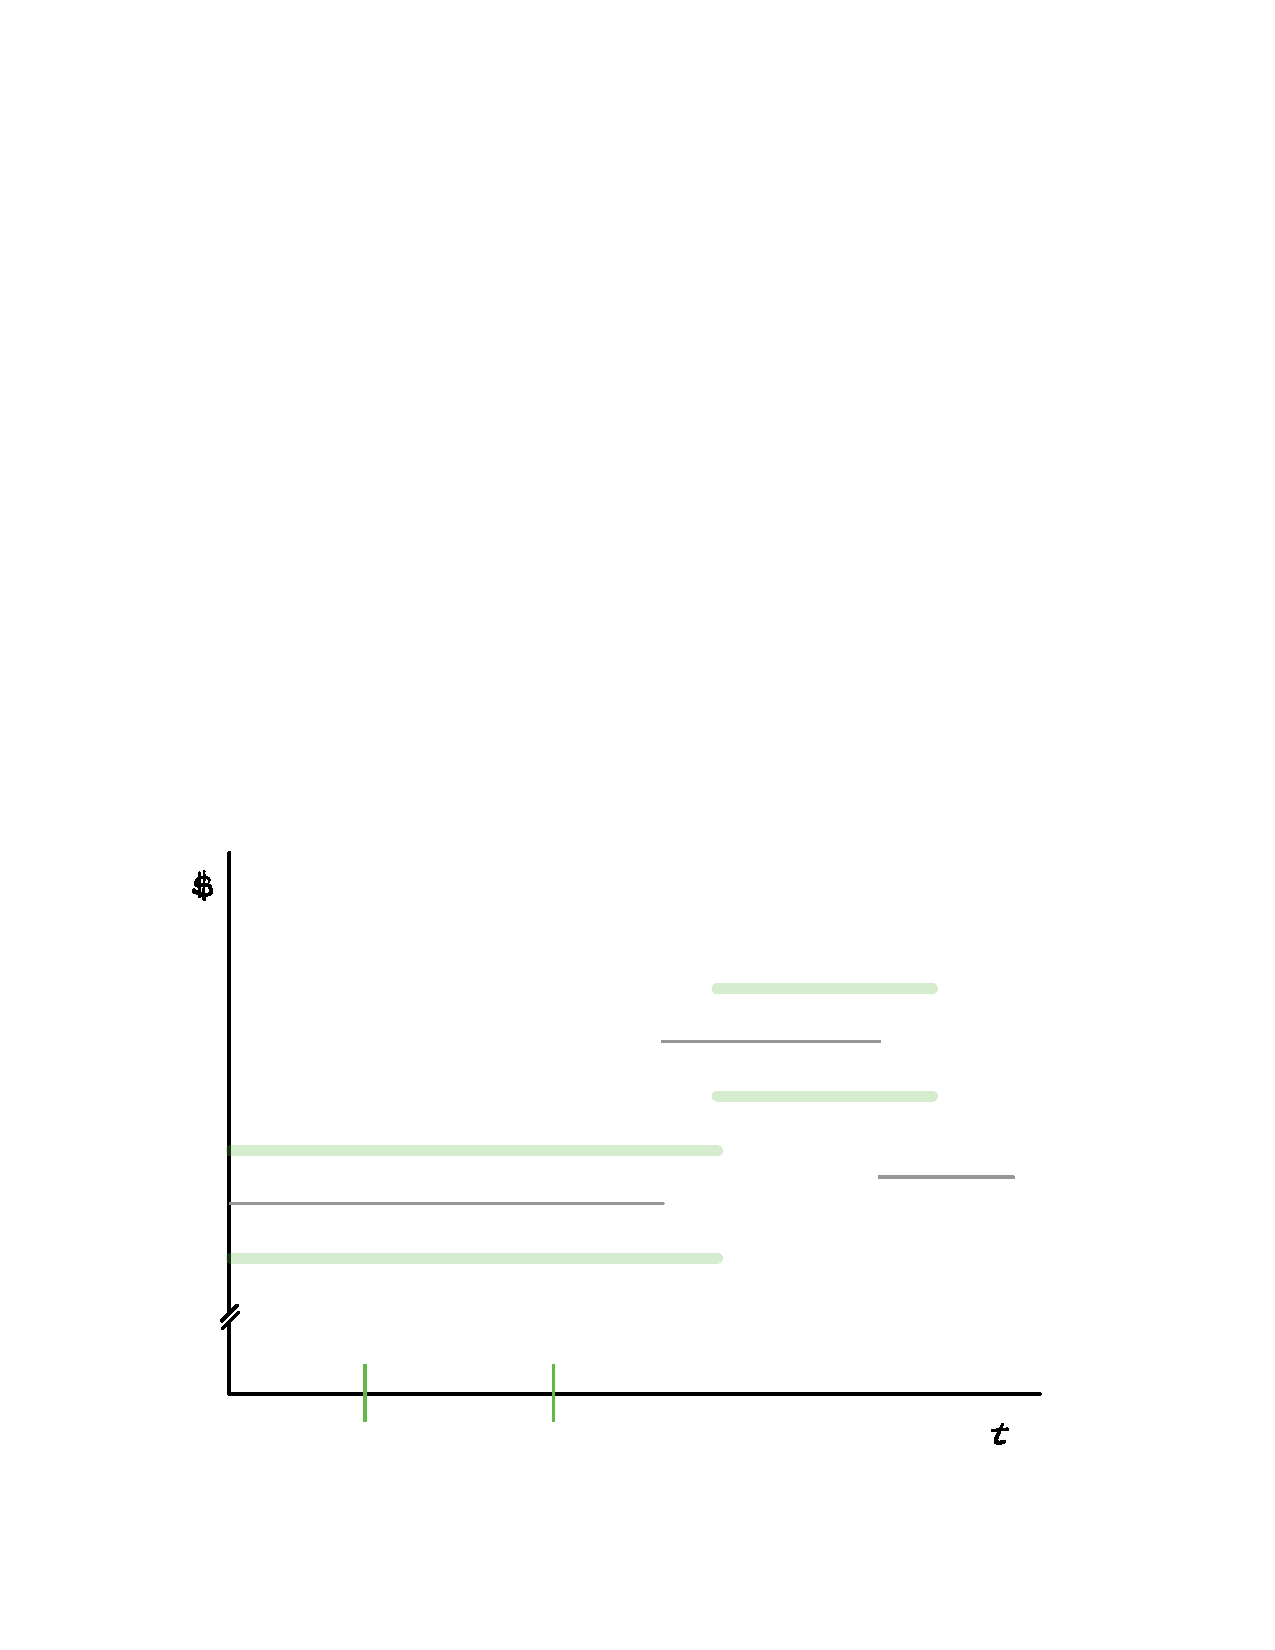
\includegraphics[width=0.7\textwidth]{img/buy_sell.pdf}
\end{figure}
}


\frame{\frametitle{Market Format 1: The CDA} 
Continuous Double Auction (CDA): 
\begin{itemize}
\item Trade can happen at \textbf{any moment} of time. 
\item Strict \textbf{price, time priority}. 
% \item Market makers: post buy/sell limit orders that remain in the book. 
% \item Takers: submit market orders to transact immediately. 
\end{itemize} 
\textbf{Trading strategies: 
}
\begin{itemize}
\item market maker (also sets a spread)
\item sniper 
\end{itemize}
\textbf{Technology strategy:}
\begin{itemize}
\item Traders can subscribe to faster (lower-latency) communication technology at a cost of $c_{speed}$ per second.
\end{itemize}
\centering 
\textbf{There is value to reacting faster to public signal} \\

}



% \frame{\frametitle{Market Format 1: The CDA} 

% \begin{enumerate}
%     \item Investor arrivals, value jumps in the CDA, sniping, profits.
%     \item Equilibrium: N-1 snipers; 1 maker with $S>0$; all fast. \hyperlink{CDA_Equil}{\beamergotobutton{Detail}}
% \end{enumerate}

% \begin{figure}
% 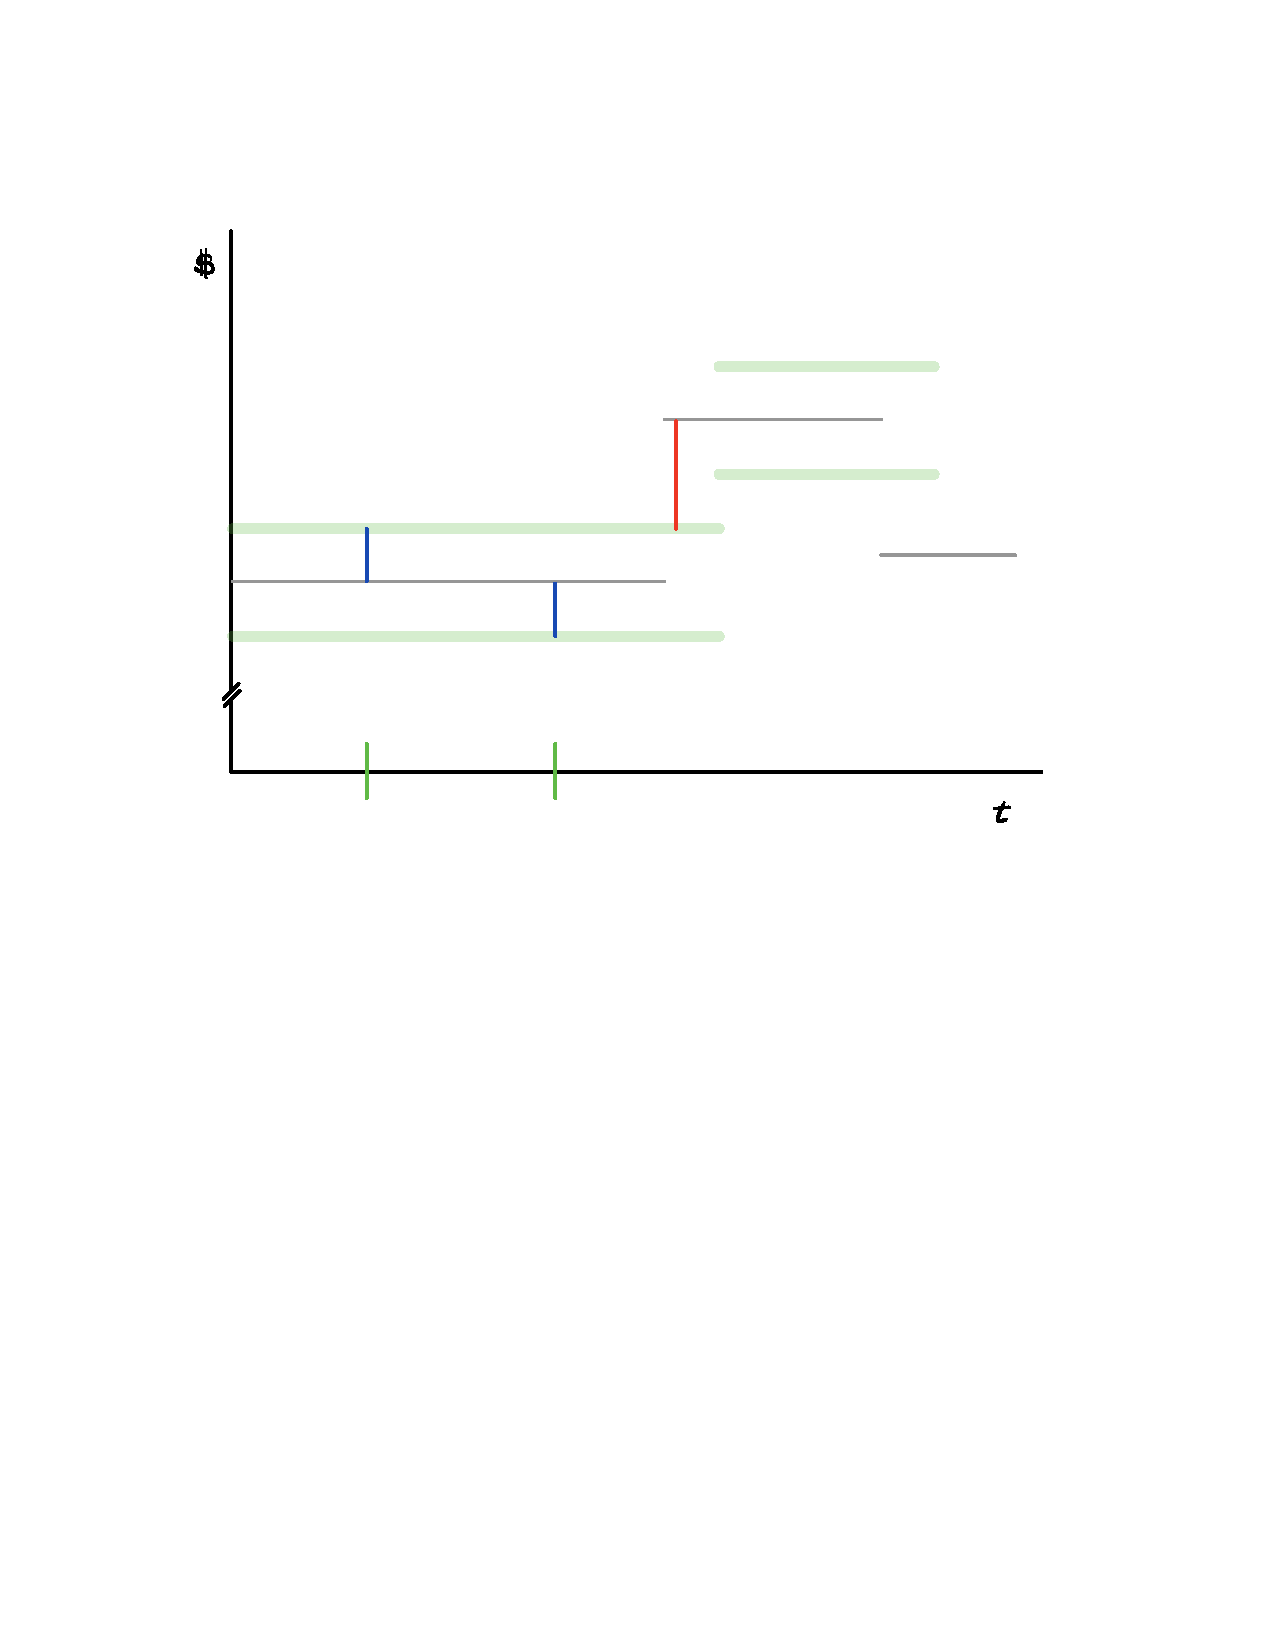
\includegraphics[width=0.6\textwidth]{img/CDA_diagram_events.pdf}
% \end{figure}
% }



% \frame{\frametitle{Market Format 1: The CDA} 
% Investor events:
% \begin{itemize}
% \item Investors' sell orders transact with the highest maker bid and buy orders transact with the lowest maker offer. 
% \item The maker with smallest spread, $s$, books profit $0.5s$ at a rate dictated by $\lambda_{I}$. 
% \end{itemize}
% Value jumps:
% \begin{itemize}
% \item At the moment of a sufficiently large positive (negative) change in the fundamental value($|\Delta V(t)| = |V(t)-V(t^{-})| > 0.5s$) snipers attempt to trade with the lowest ask (or highest bid) in the book.
% \item If this attempt is executed, we say a maker has been "sniped". Losses/gains = $|\Delta V(t)|-0.5s$ 
% \end{itemize}
% Ties are resolved randomly. \\
% }



% \frame{\frametitle{Market Format 1: The CDA} 

% Equilibrium is characterized by two zero-profit conditions. \\
% For the maker,
% \begin{equation}
%   \lambda_{I} \cdot \frac{s}{2} - 
%   \lambda_V    \cdot    \textrm{Pr}\left(J > \frac{s}{2}\right)    \cdot    E \left[J-\frac{s}{2} | J>\frac{s}{2}\right] 
%   \cdot    \frac{N-1}{N}   =   c_s, 
%   \label{eq:CDAmakerProfit}
% \end{equation}
% I.e.: expected profits from trading with investors minus the expected losses to snipers equal to the cost of buying speed services.
% }

% \frame{\frametitle{Market Format 1: The CDA} 
% For the sniper,
% \begin{align}
% \lambda_V \cdot \textrm{Pr}\left(J > \frac{s}{2}\right) \cdot E\left[J-\frac{s}{2}|J>\frac{s}{2}\right] \cdot \frac{1}{N} & = c_s, \label{eq:CDAsniperProfit}
% \end{align}
% I.e.: profits from sniping must be equal to expenditure on speed services. \\
% \vspace{5mm}
% Notice that all traders are subject to identical communication latency $\delta_{fast}$, causing the messages of all $N$ players to arrive in the exchange at the same time.
% }

% \frame{\frametitle{Market Format 1: The CDA} 
% Equilibrium in BCS environment under CDA: \\
% \begin{itemize}
% \item $N*$ traders in the market. One market maker, $N*-1$ snipers. \\ 
% \item Every trader invests in speed technology. \\
% \end{itemize}

% Rearrangement of equations \eqref{eq:CDAmakerProfit} and \eqref{eq:CDAsniperProfit} gives: 
% \begin{align}
% \lambda_I \cdot \frac{s^*}{2} & = 
% \lambda_V \cdot \textrm{Pr}\left(J > \frac{s^*}{2}\right) \cdot E\left[J-\frac{s^*}{2}|J>\frac{s^*}{2}\right] \label{eq:BCS1} \\
% \lambda_I \cdot \frac{s^*}{2} & = N^* c_s. \label{eq:BCS2}
% \end{align}

% Equation \eqref{eq:BCS1} determines $s^*$ and Equation \eqref{eq:BCS2} determines $N^*$. \\
% \vspace{5mm}

% Intuition: The cost of speed, purchased by all traders, is borne entirely by investors via market spread. 
% }

%%%%%%%%%%%%%%%%%%%%%%%%%%%%%%%%%%%%%%%%%%%%%%%%%%%%

\frame[label={FBA}]{\frametitle{Market Format 2: The FBA} 
Frequent Batch Auction (FBA): 
\begin{itemize}
\item Trading day is divided in \textbf{many uniform price double auctions}:
\item Trade does NOT happen at any moment of time, but \textbf{periodically} (say, each tenth of a second), with a batching period for each auction.
\item At the end of the batching period, supply and demand cross and \textbf{market clears}. 
 \item Strategy space is the same as in the CDA. 
\end{itemize}

\begin{figure}
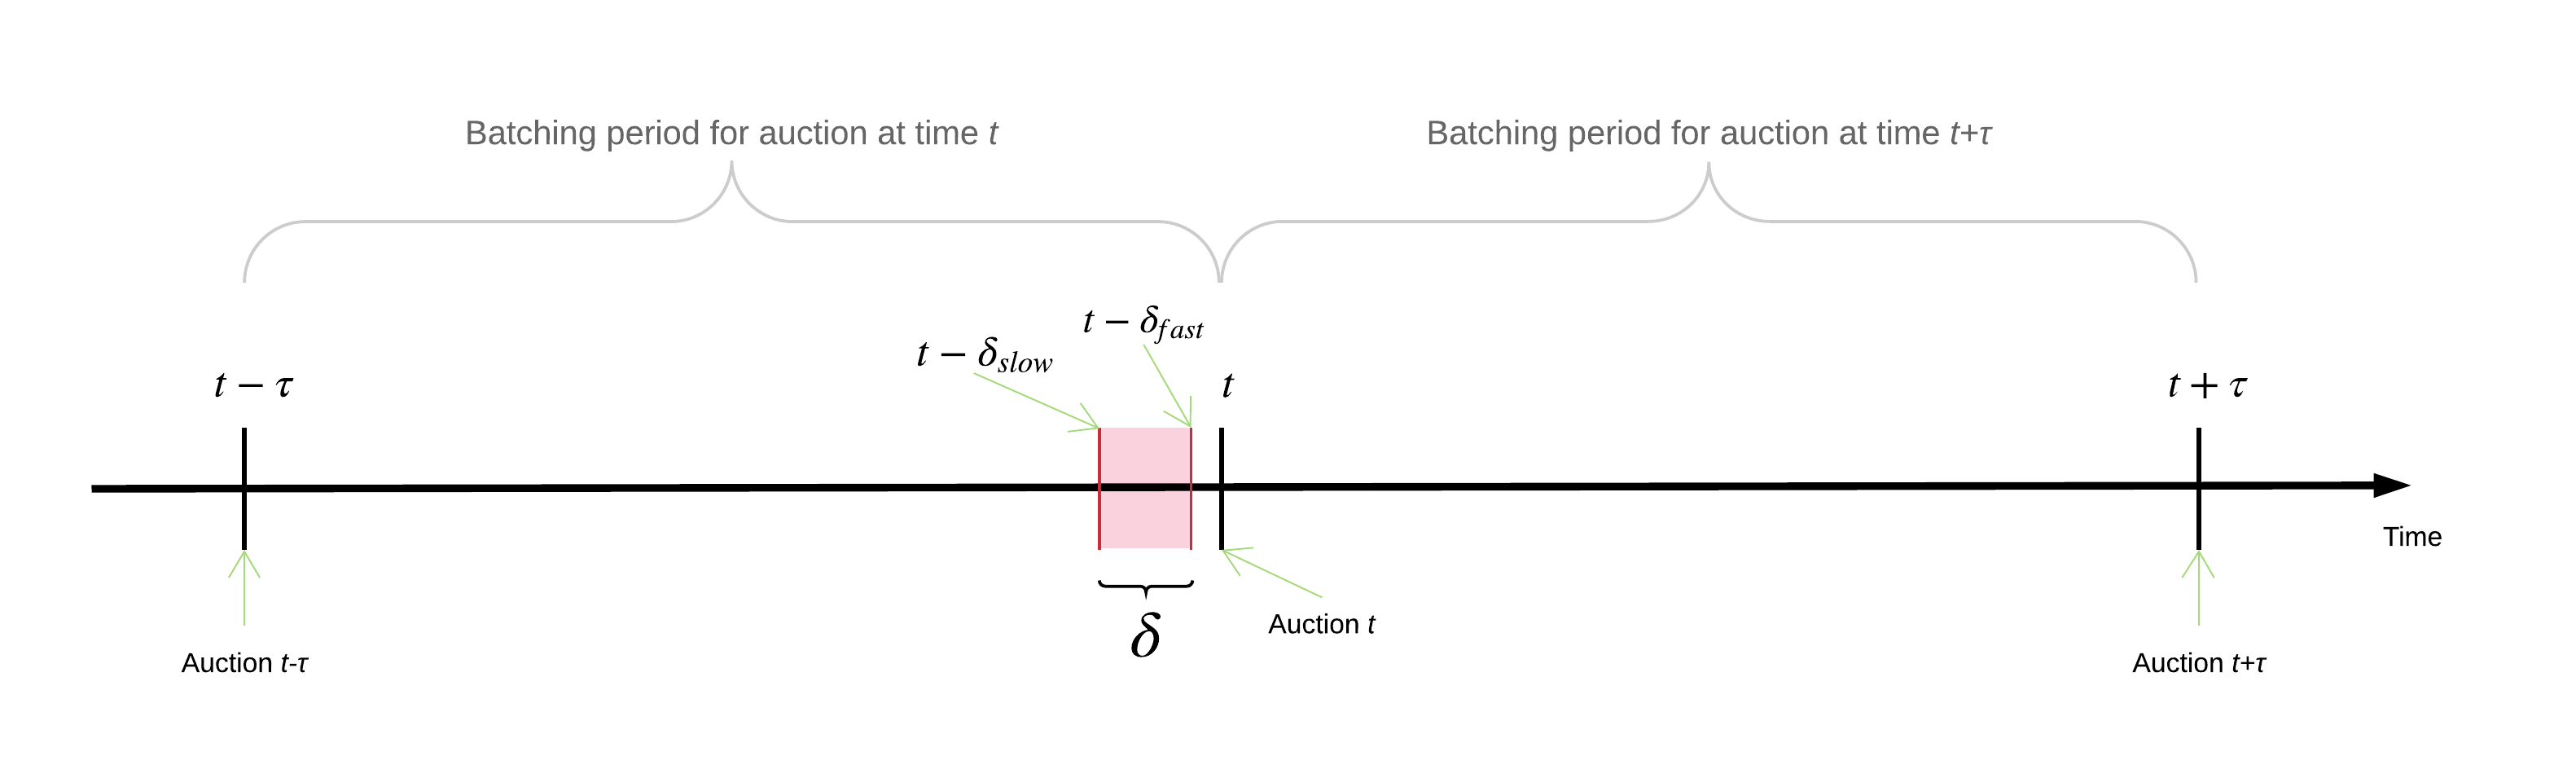
\includegraphics[width=0.8\textwidth]{img/timing_FBA.png}
\caption{\label{fig:FBAtiming}Timing in the FBA format (adapted from Budish et al. (2015)).}
\label{fig:fbaDiagram}
\end{figure}
}


\frame{\frametitle{Market Format 2: The FBA} 
Equilibrium: No snipers, everyone is \textit{maker} with $S=0$; all slow.
\hyperlink{FBA_Equil}{\beamergotobutton{}}
\begin{figure}
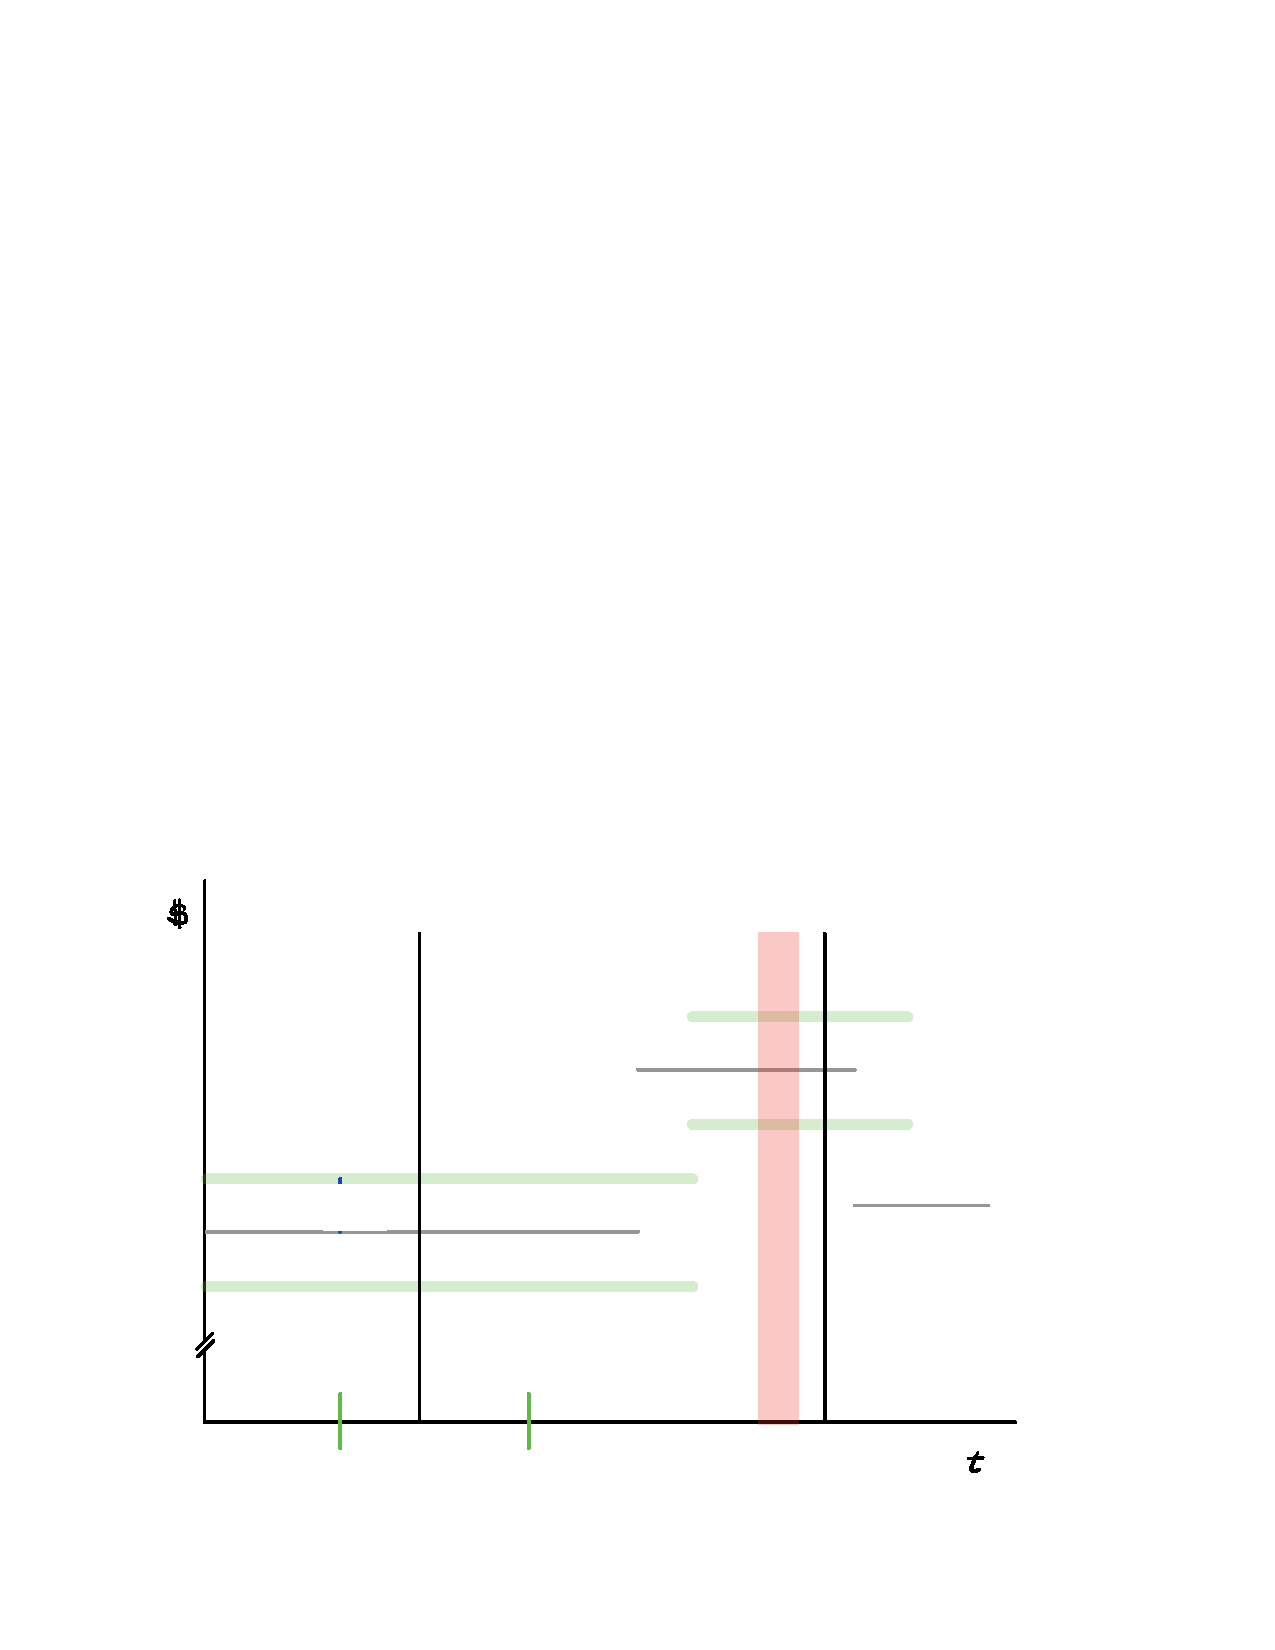
\includegraphics[width=0.7\textwidth]{img/FBA_diagram_events.pdf}
\end{figure}
}



%%%%%%%%%%%%%%%%%%%

\frame{\frametitle{Experiment} 
Choice Space: \\
\newline
1 Human subjects choose between 3 algos:
\begin{enumerate}
\item Out: stay out of the market
\item Maker: Post buy/sell orders at $V \pm s/2$, can freely update $s$.\\ 
With lag $\delta$, bot updates when $V$ jumps.\\ 
\item Sniper: Try to pick off stale quotes when $V$ jumps.
\end{enumerate}  

\vspace{8mm}
2 Speed subscription: 
\begin{itemize}
\item at flow cost $c>0$, reduce latency $\delta_{slow}$ to $\delta_{fast}$. ($\delta_{slow} > \delta_{fast}$) \\
\end{itemize}
}

\frame{\frametitle{Treatments, Sessions}
\begin{itemize}
\item \textbf{Six treatments} $\{CDA,FBA\} \times \{C1,C2,C3\}$.
\item \textbf{Between-subjects} design
\item Market or \textbf{Group size = 6}; partner matching.
\item A session = \textbf{eight trading periods} of four minutes each 
\item Data for 24 markets or groups (4 groups per treatment, 12 sessions total).
\item Initial endowment: 20 ECUs; Exchange rate: 2 ECUs = 1 USD; 
\item Subjects \textbf{paid for one randomly chosen} period plus 7 USD. 
\item  Summary information between periods.
\item Sessions conducted at the LEEPS Laboratory at UCSC.
\end{itemize}
}

\frame{\frametitle{Treatments, Sessions}
\begin{table}[]
\centering
\begin{tabular}{lccc}
\hline
                                        & Config 1              & Config 2              & Config 3              \\ \hline
Parameters:                             &                       &                       &                       \\ 
%\multicolumn{1}{|c|}{
$ \ \ \ \ \ \lambda_{I}$ & 1/3                   & 1/5                   & 1/2                   \\ 
%\multicolumn{1}{|c|}{$ \\ \lambda_{V}$} 
$ \ \ \ \ \ \lambda_{V}$ & 1/4                   & 1                     & 1                     \\ 
%\multicolumn{1}{|c|}{$ \\ c_{speed}$} 
$ \ \ \ \ \  c_{speed}$   & 0.01                  & 0.01                & 0.022                 \\ 
Number of trading periods               & 8                     & 8                     & 8                     \\ 
Trading period length (secs)            & 240                   & 240                   & 240                   \\ 
                                        & 		 				& 	 					&  						\\ 
Groups per treatment            & 4                 & 4                 & 4                \\ \hline
\end{tabular}
\end{table}
}



\frame{\frametitle{CDA User Interface}
%\begin{itemize}\item 
%\centering
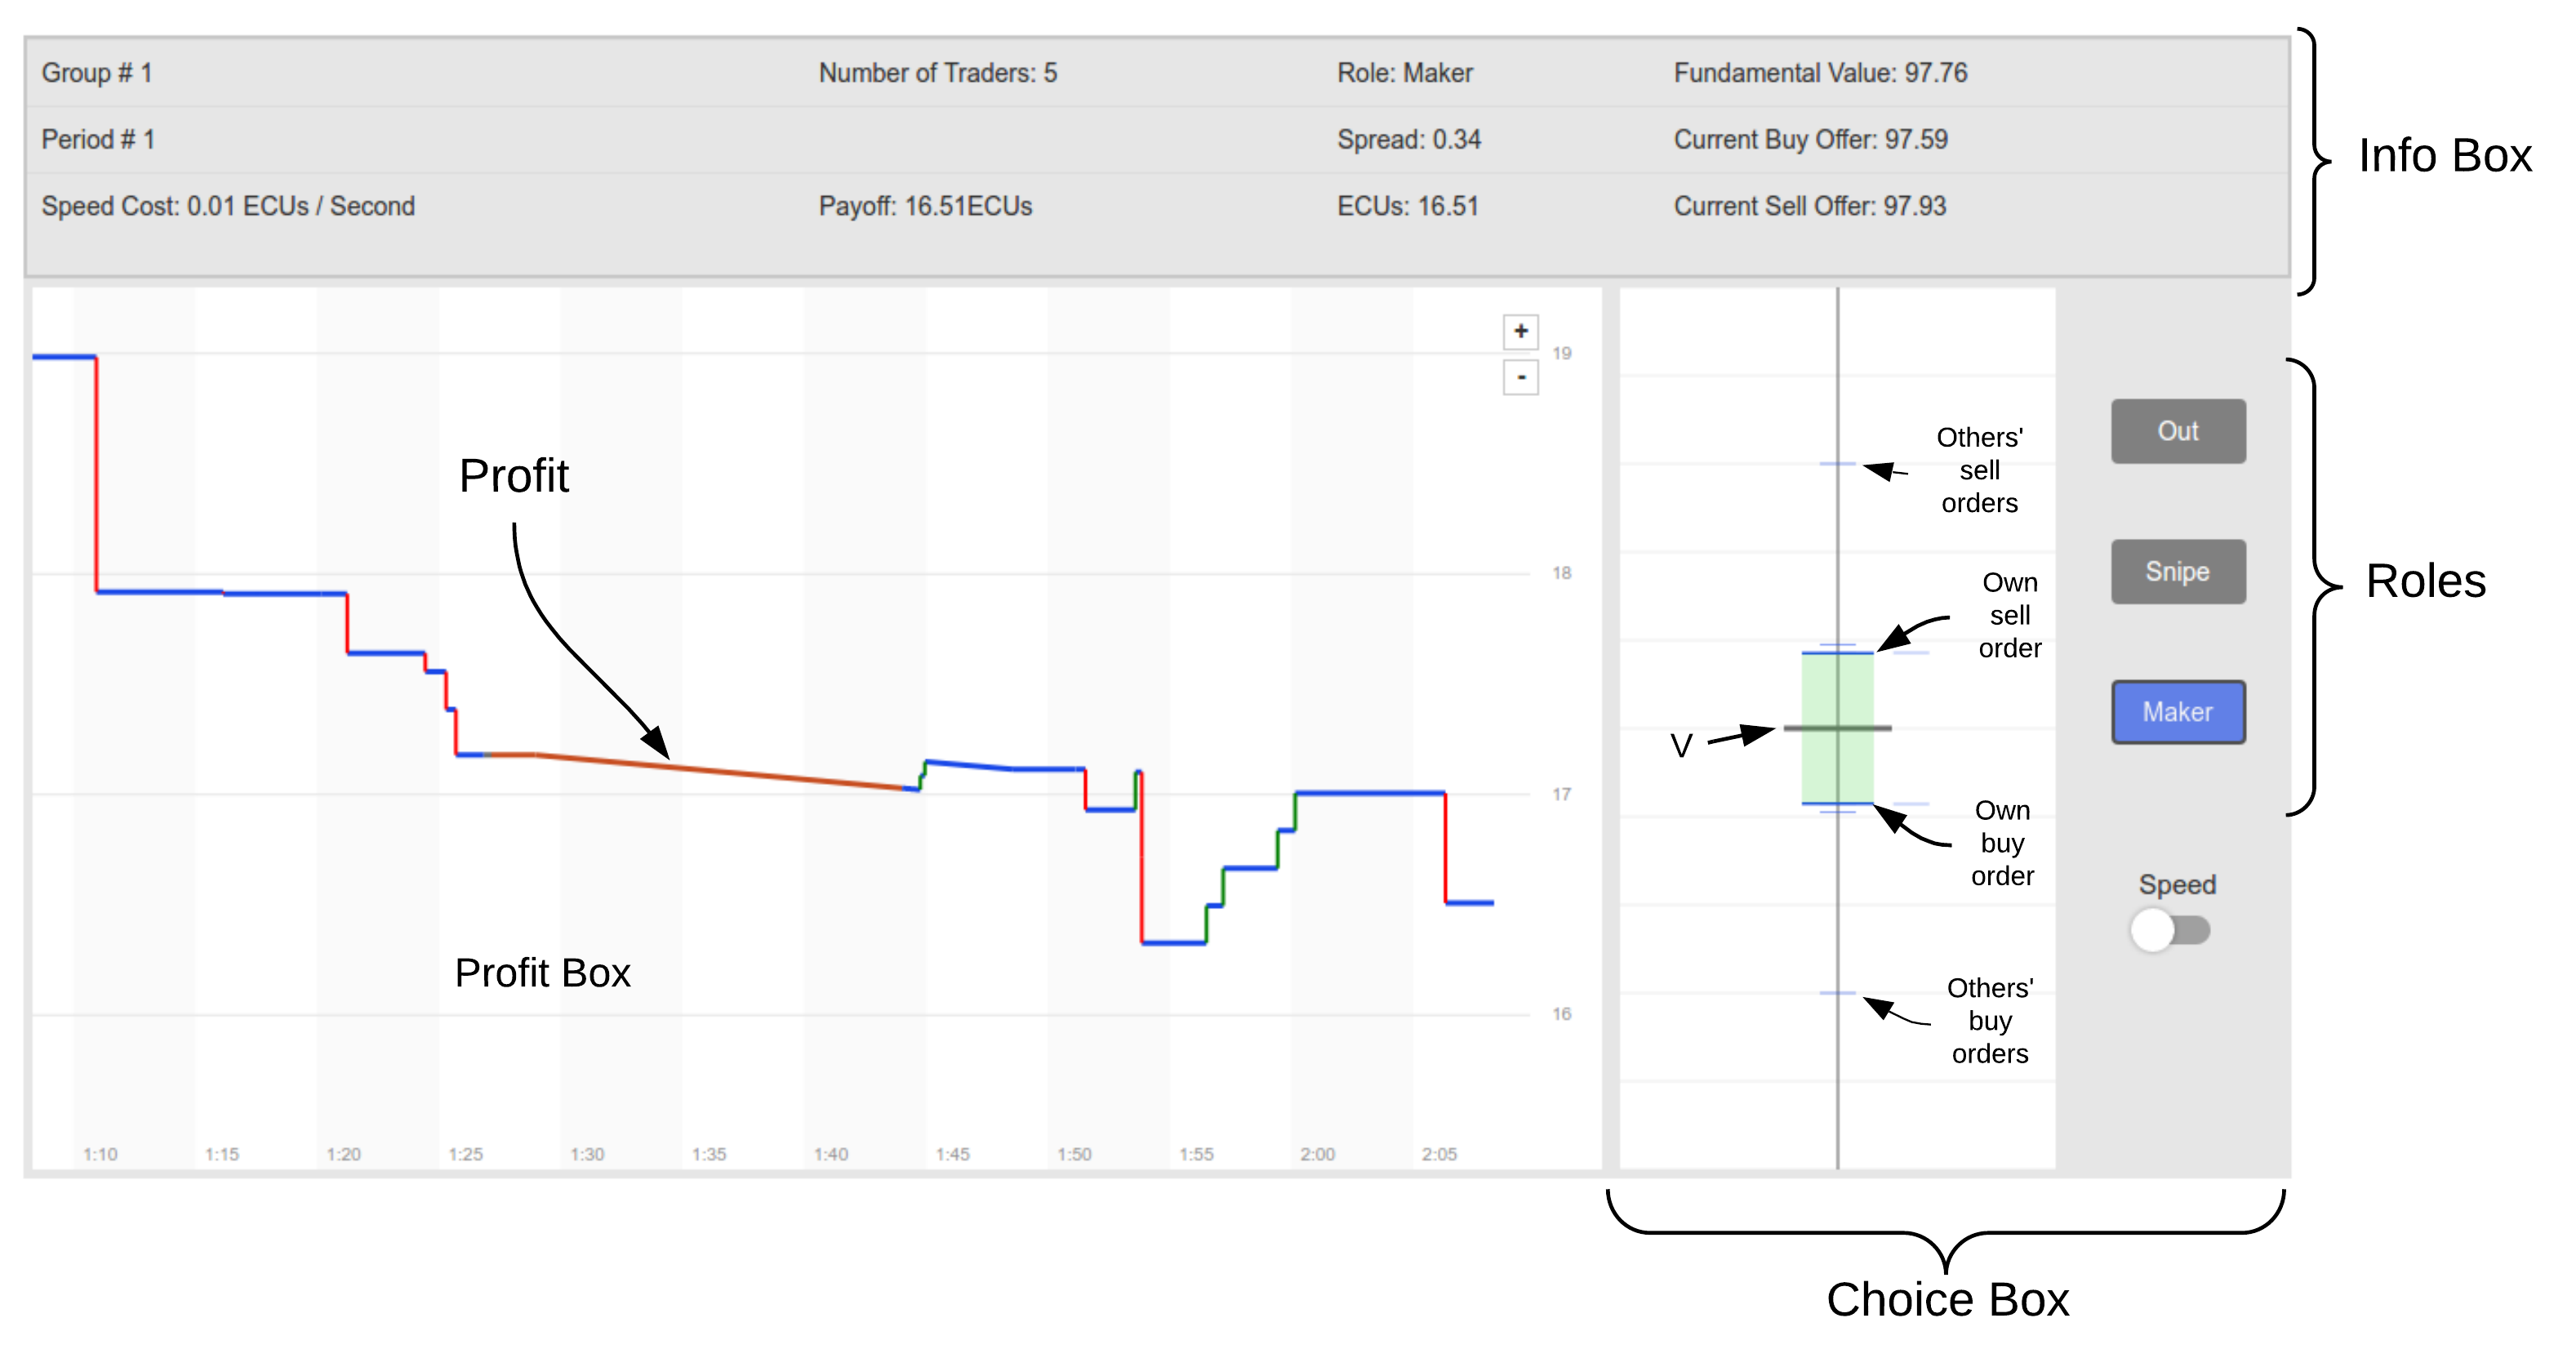
\includegraphics[width=1.06\textwidth]{img/UI-CDA_with_labels.png}
}

\frame{\frametitle{FBA User Interface}
%\begin{itemize}\item 
%\centering
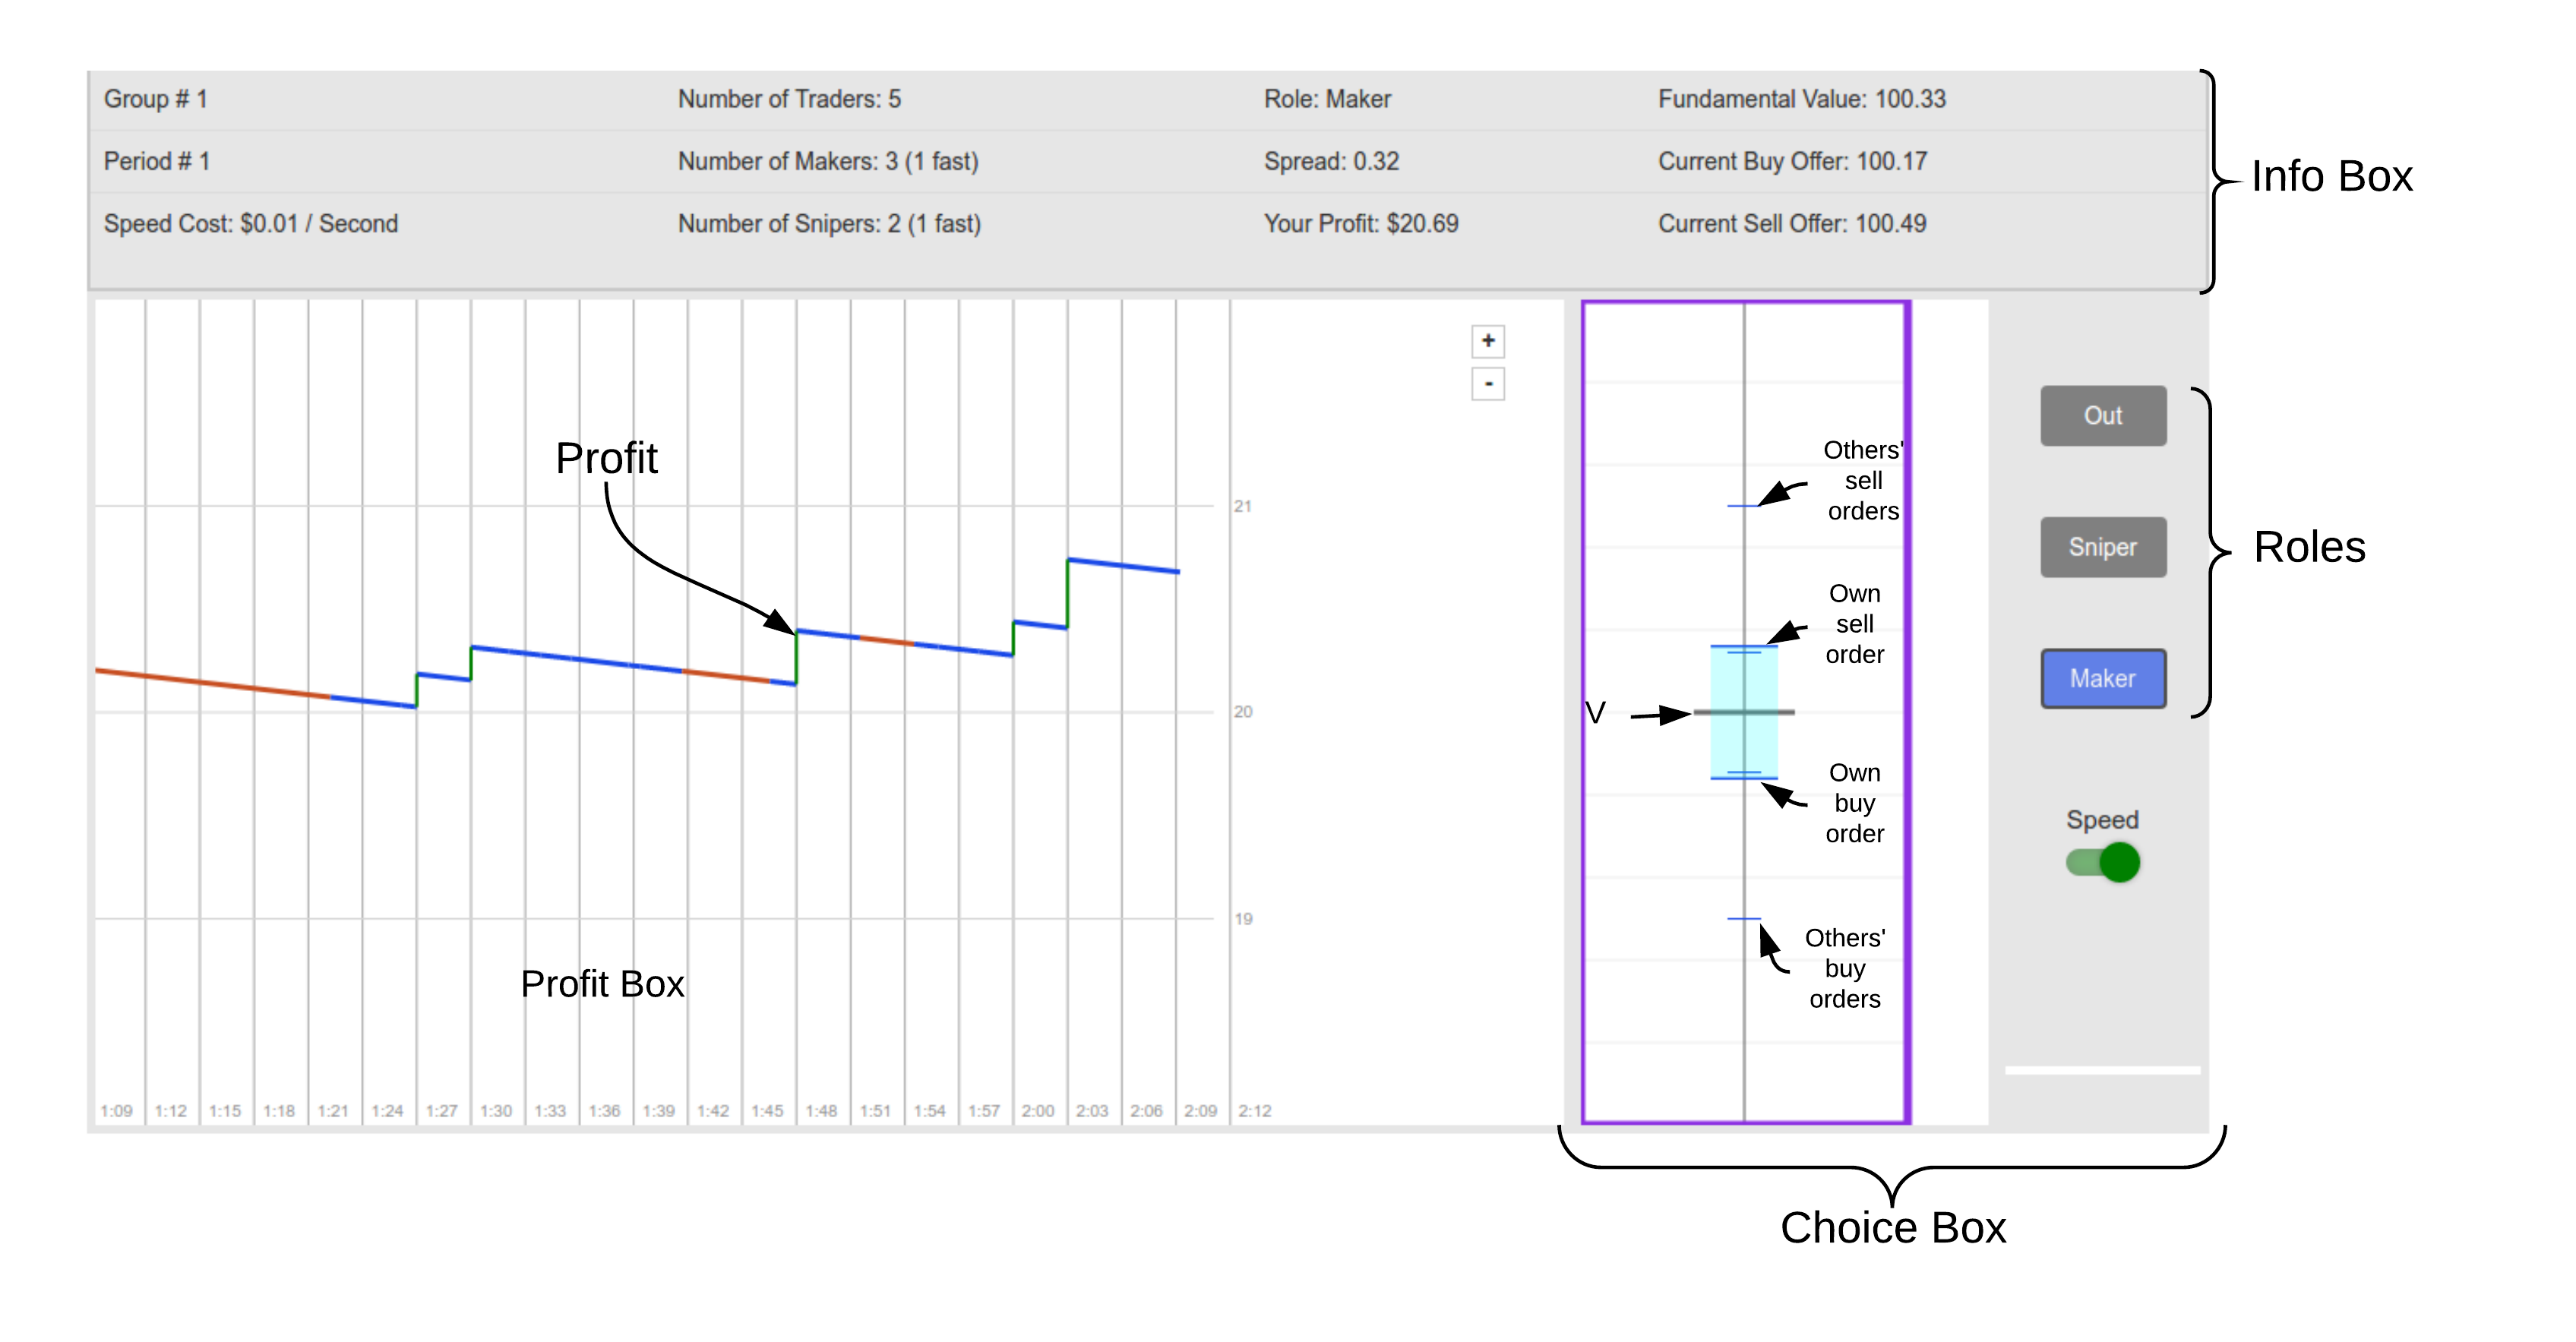
\includegraphics[width=1.06\textwidth]{img/UI-FBA.png}
}



\frame{\frametitle{Results: Summary} 

In choice data, the FBA exhibits:
\begin{itemize}
\item more traders choose to act as makers
\item fewer choose to act as snipers
\item fewer choose to purchase speed services
\item smaller market spreads 
\end{itemize}

In market level data, the FBA:
\begin{itemize}
\item reduces the volatility of transaction prices and spread
\item enhances price efficiency
\item results in more stable trader choices
\end{itemize}
}

% %3.1 Subject choices
% \frame{ 
% \begin{figure}
% 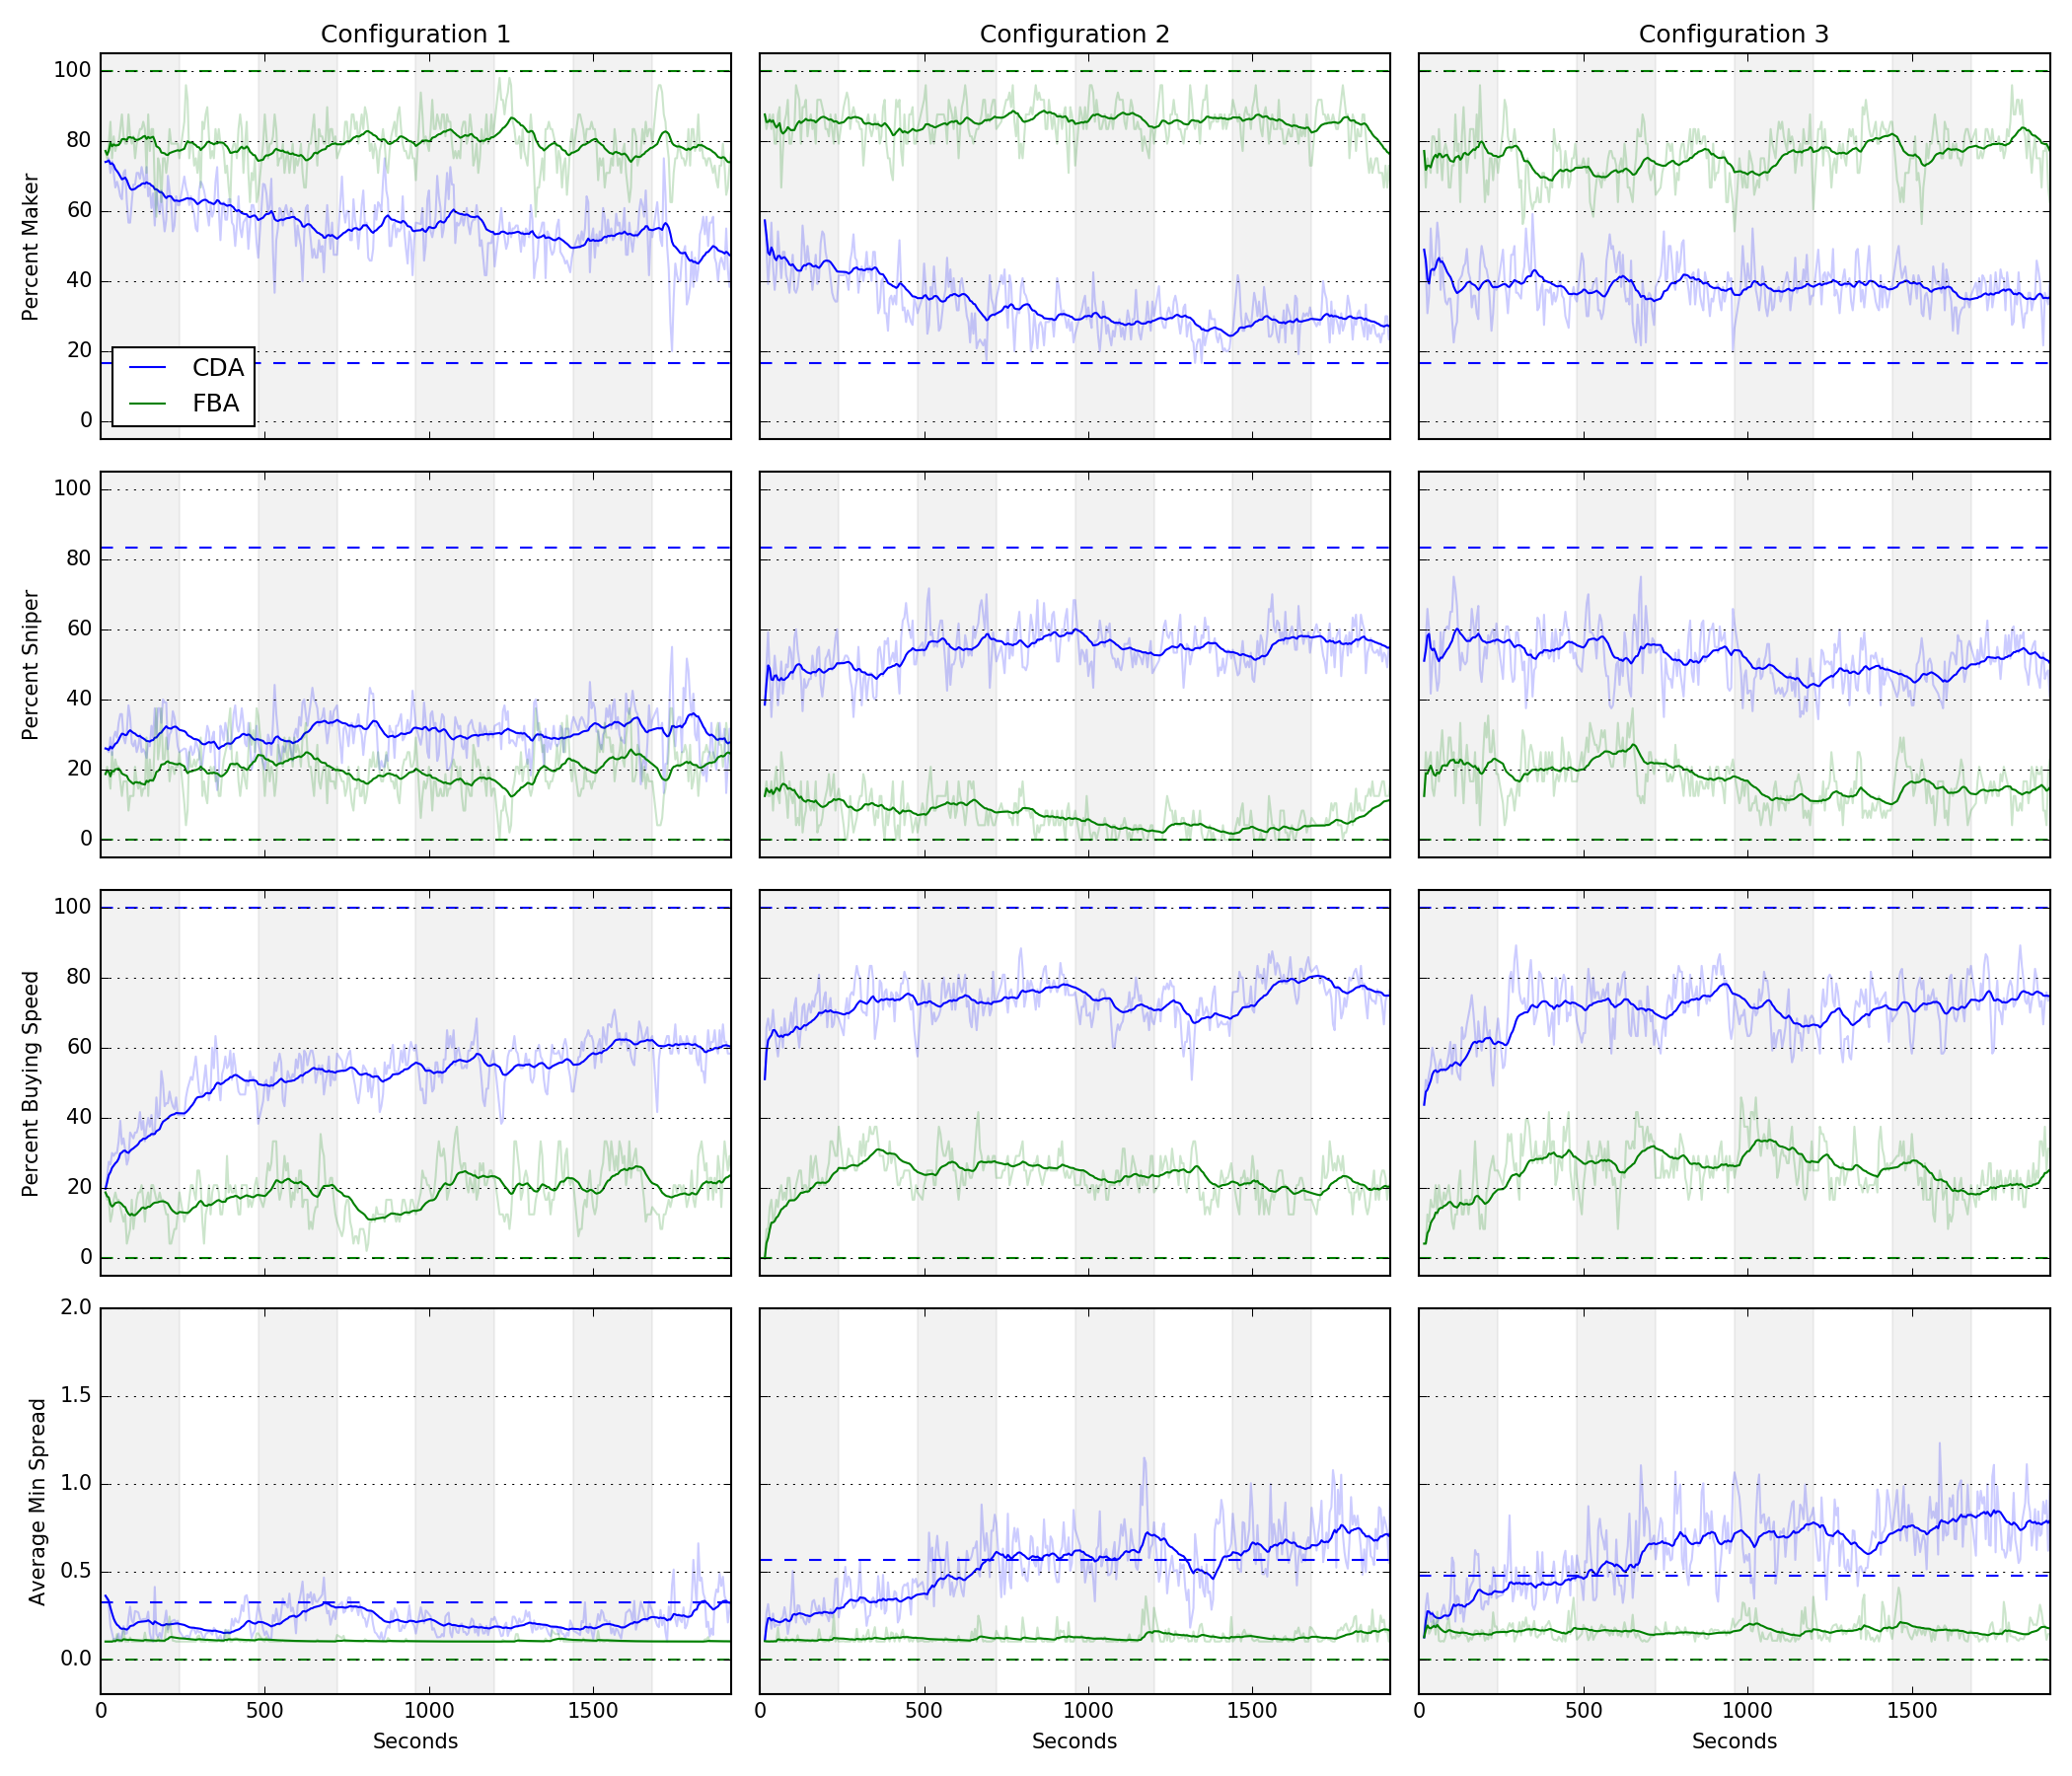
\includegraphics[width=0.70\textwidth]{img/allPlots.png}
% \end{figure} 
% Rows: \% Maker, \% Sniper, \% Speed, Spread \\
% Cols: Market Configs 1, 2, 3.
% }

\frame{\frametitle{Results: Summary Statistics for \textbf{Choices}} 
\begin{table}[]
\centering
%\caption{My caption}
\scalebox{.8}{
\begin{tabular}{llcccccc}
\hline
&& \multicolumn{2}{c}{ Config. 1 } & \multicolumn{2}{c}{ Config. 2 } & \multicolumn{2}{c}{ Config. 3 } \\
                    %  &             & C1 & C1 & C2 & C2 & C3 & C3 \\
                     &             & CDA      & FBA    & CDA      & FBA    & CDA      & FBA    \\ \hline
Making (\%)        &             &          &        &          &        &          &        \\
                     & Experiment  & 54    & 78.1  & 30.2    & 78.8  & 40.1    & 72.9 \\
                     & Equilibrium & 16.7    & 100 & 16.7    & 100 & 16.7    & 100 \\
Sniping (\%)         &             &          &        &          &        &          &        \\
                     & Experiment  & 31    & 20.8  & 58.1    & 14.5  & 49.5    & 14 \\
                     &  Equilibrium & 83.3    & 0   & 83.3    & 0  & 83.3    & 0   \\
Speed (\%)            &             &          &        &          &        &          &        \\
                     &  Experiment & 56.1    & 19.7  & 69    & 31.7  & 69.2    & 20.7 \\
                     & Equilibrium & 100   & 0  & 100   & 0   & 100  & 0   \\
Min. Spread &             &          &        &          &        &          &        \\
                    &  Experiment & 0.226    & 0.103  & 0.677    & 0.179  & 0.709    & 0.147  \\
                     & Equilibrium & 0.324    & 0 & 0.566    & 0  & 0.475    & 0  \\ \hline
\end{tabular}}
\end{table}
\begin{footnotesize}
% Panel (b) reports the average percentage of subjects acting as market makers, snipers, average percentage of subjects purchasing speed services, and the average minimum spread posted by market makers.
\end{footnotesize}
}

\frame{\frametitle{Results: Summary of \textbf{Market Stats}} 
\begin{table}[]
\centering
\scalebox{.6}{
\begin{tabular}{llcccccc}
\hline
&& \multicolumn{2}{c}{ Config. 1 } & \multicolumn{2}{c}{ Config. 2 } & \multicolumn{2}{c}{ Config. 3 } \\
                     &             & CDA      & FBA    & CDA      & FBA    & CDA      & FBA    \\ \hline
$Std(P_t-P_{t-1})$        &             &          &        &          &        &          &        \\
                     &  Experiment & 2.51 & 0.561 & 4.62 & 1.00  & 6.68 & 1.11 \\
                     & Equilibrium & 0.241    & 0.289 & 0.276    & 0.327  & 0.235    & 0.430  \\
$Std(MinSpread)$         &             &          &        &          &        &          &        \\
                     &  Experiment & 0.204 & 0.0235 & 0.536 & 0.144 & 0.394 & 0.127 \\
                     & Equilibrium & 0    & 0 & 0    & 0  & 0    & 0  \\
Status Changes            &             &          &        &          &        &          &        \\
                    & Experiment & 20.5 & 6.26 & 31.6 & 6.26 & 17.0 & 7.34 \\
                     & Equilibrium & N/A   & 0 & N/A    & 0  & N/A    & 0  \\
$RMSD(P_t-V_t)$ &             &          &        &          &        &          &        \\
                    &  Experiment  & 0.347 & 0.212 & 0.512 & 0.410 & 0.460 & 0.381 \\
                     & Equilibrium & 0.223    & 0.136 & 0.329    & 0.211  & 0.372    & 0.276  \\ 
Transactions &             &          &        &          &        &          &        \\
                    & Experiment & 156 & 85.2 & 172 & 99.3 & 248 & 134 \\
  					 & Equilibrium & 106 & 80 & 100 & 48 & 147 & 120 \\
Period Profits &             &          &        &          &        &          &        \\
                    & Experiment  & .0869 & .435 & .603 & .372 & 4.31 &  1.52 \\
                     & Equilibrium & 0    & 0 & 0    & 0  & 0    & 0  \\ \hline
\end{tabular}}
\end{table}
}



\frame{\frametitle{Results: Regressions Analysis} 
To quantify treatment effects, we estimate the following model:
\begin{align}
y_{g,t}= \sum_{j=1}^{3}[\alpha_{j}Cj_{g,t}+\gamma_{j}Cj \times FBA_{g,t}] + \epsilon_{g,t},
\end{align}
where $y_{g,t} \hspace{0.1cm} \epsilon \hspace{0.1cm} \{Maker_{g,t}, Sniper_{g,t}, Speed_{g,t}, MinSpread_{g,t}\}$ is indexed by group and time, $Cj$ is a dummy variable for market configuration $j \hspace{0.1cm} \epsilon \hspace{0.1cm}$ \{1,2,3\} and $Cj \times FBA_{g,t}$ is the dummy variable indicating the interaction between configuration $j$ and the FBA format.
}

\frame{\frametitle{Results: Regressions Analysis} 
\begin{figure}
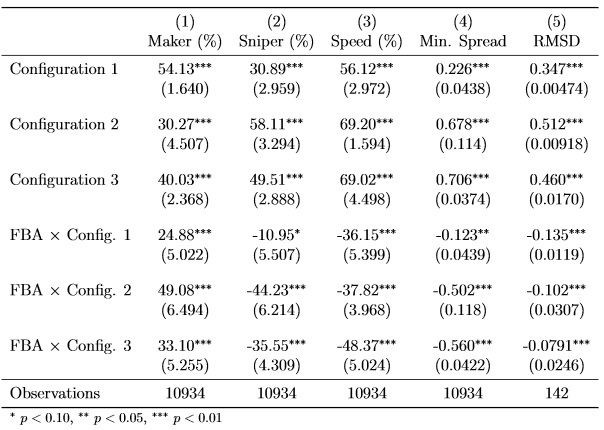
\includegraphics[width=0.75\textwidth]{img/Reg1_KL.jpg}
\end{figure} 
\begin{footnotesize}
\end{footnotesize}
}

\frame{\frametitle{Results: Regressions Analysis} 
\begin{enumerate}
    \item Equilibrium behavior is rejected.
    \item However, the relative comparative statics of the two formats predicted by the model is confirmed in the data.
    \item Relative to the CDA, the FBA exhibits:
\begin{itemize}
\item more makers (higher liquidity)
\item fewer snipers
\item fewer purchases of socially wasteful speed technology
\item lower market spreads
\item lower RMSDs (higher efficiency)
\end{itemize}

\end{enumerate}
}


%%%%%%%%%%%%%%%%%%%%%%%%%%

\frame{\frametitle{Conclusions}
\begin{itemize}
\item Differences between FBA and CDA in the lab are consistent with comparative statics of the BCS model. 
\item FBA outperforms CDA:
\begin{enumerate}
\item less \textbf{predatory} trading behavior.
\item less \textbf{wasteful investments} in technology.
\item lower \textbf{transacting costs} (market spread)
\item lower \textbf{volatility}, 
\item higher market \textbf{stability}
\end{enumerate}
% \item FBA outperforms CDA in transaction costs (BCS environment). Effect sizes tend to be smaller than predicted.
% \item Predatory behavior (sniping) is more prevalent in CDA than in FBA.
% \item More turbulent markets in terms of stock value volatility (Config 2 and 3) exhibit difference between CDA and FBA formats more clearly  perhaps because more V-jump events.
\item Ongoing and future research (larger project w/ PC, DF, AO)
\begin{itemize}
    \item More realistic environments.
    \item Other market formats: IEX, Kyle-Lee, etc. 
    \item Multiple formats.
\end{itemize}


\end{itemize}
}


\frame{
\centering
{\huge Thank You} \\  
{\small \url{kristian@ucsc.edu} }
\\ 
\\
\hyperlink{start}{\beamerbutton{\tiny{Back to start} \Bicycle}}

}



\frame{\frametitle{More on Motivation: the HFT Debate} 
\hypertarget{motivationDetail}{}

\begin{itemize}
\item The CDA/CLOB has a \textbf{built-in design flaw} (Budish et al. 2015). 
\item Huge \textbf{rewards}  for traders that can react to information a nanosecond \textbf{faster} than others and exploit stale orders. 
\item This generates an \textbf{arms race} around expensive faster communication technology.
\item The outcome: a \textbf{massive prisoner's dilemma}
\item Are there other market rules that undo the negative incentives built-in the CDA? Yes: \textbf{FBA}, IEX, Flow markets, etc.

\item \textbf{Existing data} is insufficient to resolve the debate, as data come from a single exchange format. 

\item \textbf{Experimentation} allows us to generate evidence on the relative performance of market alternatives.	

\end{itemize}
}

%In March 2014, New York City Attorney General Eric Schneiderman launched a probe of HFT-related practices; so far he has served subpoenas on the largest HFT firms, exchanges and banks operating dark pools and 
% filed a lawsuit against Barclays, alleging that the bank illicitly operated its dark pool in ways to favor HFT. 
% In June 2016, the U.S. Securities and Exchange Commission approved a plan put forth by IEX, a new trading venue, to delay all incoming orders with the intention of reducing the advantage of HFT firms. 
%In July 2016, India?s regulators announced plans to create similar ?speed bumps? for their major financial markets. Regulators around the world are contemplating similar moves.



\frame[label={CDA_Equil}]{\frametitle{Market Format 1: The CDA} 

Equilibrium in BCS environment under CDA:
\begin{itemize}
\item Finite numbers of participants $N^*$
\item All $N$ traders purchase fast communication technology
\item Only one trader plays market maker 
\item $N-1$ are snipers.
\item Free entry. Every trader earns zero profits. 
\item The cost of speed, purchased by all traders, is borne entirely by investors via market spread: \item \textbf{$s^*>0$, $\lambda_I \frac{s^*}{2} = N^* c_s$} 

\end{itemize}

}


\frame[label={FBA_Equil}]{\frametitle{Market Format 2: The FBA} 


\vspace{5mm}

Equilibrium of the FBA in the BCS environment: \\
\begin{itemize}
\item Everyone is a \textit{slow maker} with zero spread ($s^*=0$). 
\item There are no sniper
\item No one purchases fast technology.
\end{itemize}

... This eqm holds if the batching period is substantially larger than default communication latency.

}

\frame{\frametitle{Market Format 2: The FBA} 

Technically, the condition is (Budish et al., 2015) :
\begin{align} 
\label{eq:BCSFBA}
\frac{\delta}{\tau} \cdot \lambda_V E\left[J | J>0\right] < c_s
\end{align}
I.e., there is no incentive for traders to take the role of a fast sniper in the FBA.
}


\frame{\frametitle{Transitory Market Dynamics}
To understand the dynamics of the market and the possible effects of transitory changes in the environment on subjects' decisions, we fit a vector autoregression of the form:
\begin{equation}
\mathbf{y}_{t}=\mathbf{a}+\mathbf{\Phi y}_{t-1}+\varepsilon_{t}
\end{equation}
\begin{equation}
\mathbf{y'}_{t}=[\%Sniper_{t}, \%Speed_{t}, MinSpread_{t}, Turbulence_{t}]
\end{equation}
}



\frame{\frametitle{Estimates of the constrained VAR(1)}
\begin{figure}
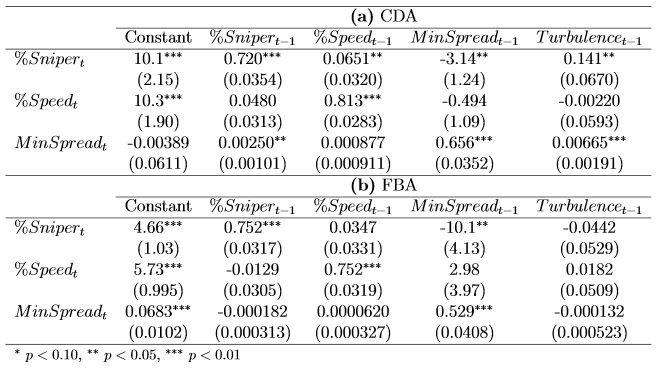
\includegraphics[width=0.75\textwidth]{img/Reg2_KL.jpg}
\begin{footnotesize}
\caption{Standard errors are reported in parentheses. Panel (a) reports CDA estimates and panel (b) 
reports FBA estimates.}
\end{footnotesize}
\end{figure} 
\begin{footnotesize}
The results show that very-short term, innovations in market conditions impact behavior in the CDA, while such effects of transient market changes do not exist in the FBA.
\end{footnotesize}
}


\frame{\frametitle{Transitory Market Dynamics}
\begin{figure}
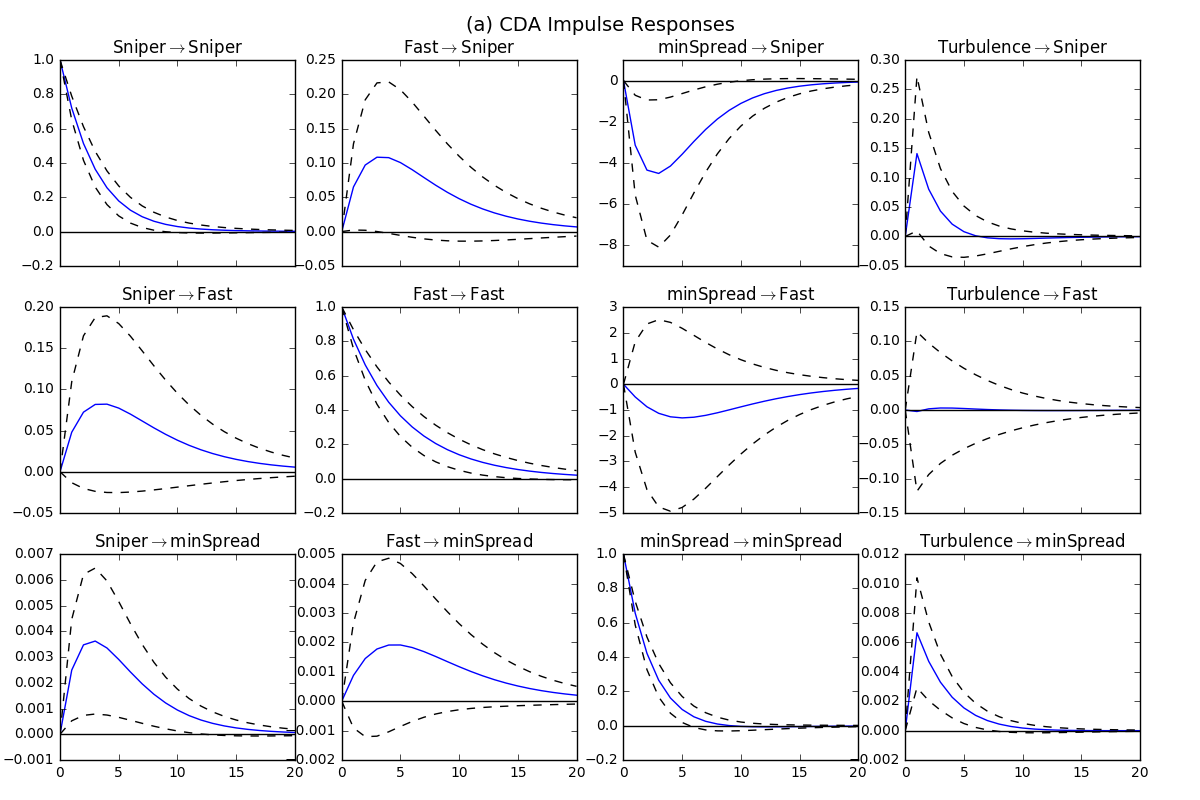
\includegraphics[width=0.80\textwidth]{img/irfCDA.png}
\caption{Unit impulse responses for the estimated VAR under CDA.}
\end{figure} 
}

\frame{\frametitle{Transitory Market Dynamics}
\begin{figure}
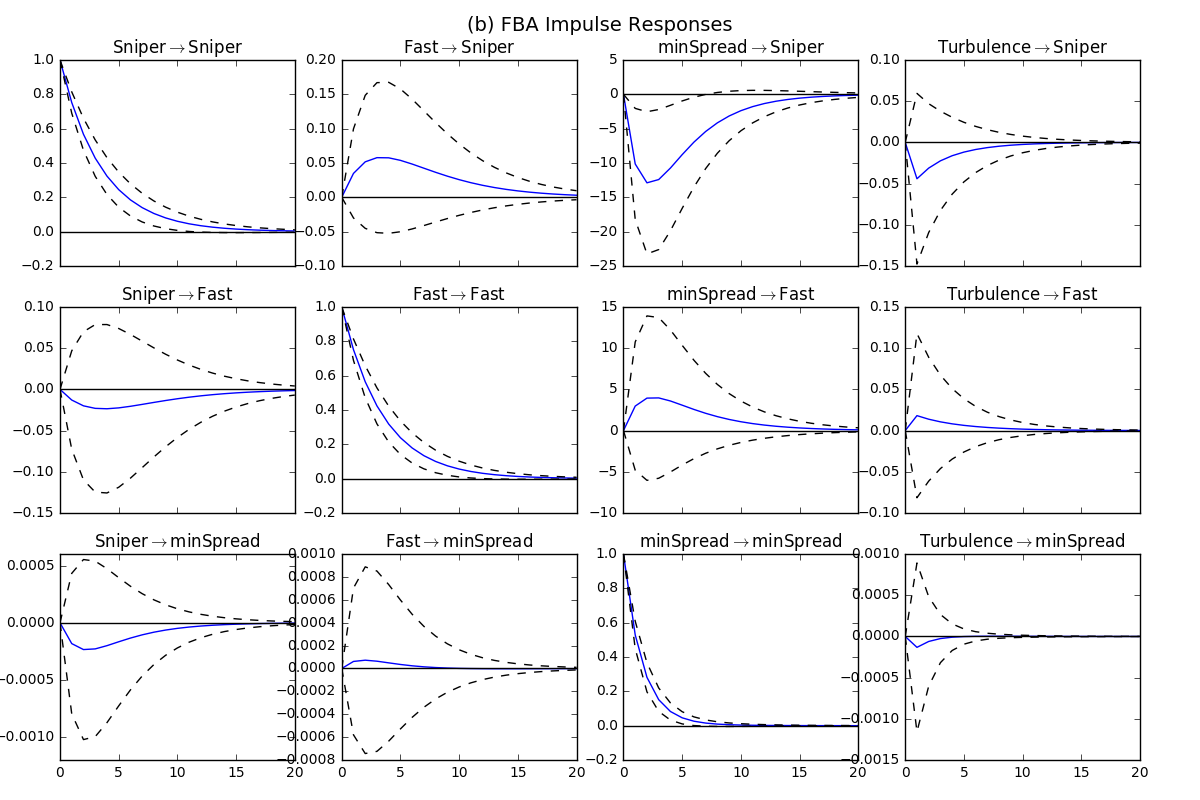
\includegraphics[width=0.80\textwidth]{img/irfFBA.png}
\caption{Unit impulse responses for the estimated VAR under FBA.}
\end{figure} 
}




\end{document}



